\documentclass{beamer}
\usepackage{textpos}
\setlength{\TPHorizModule}{1cm} % Horizontale Einheit
\setlength{\TPVertModule}{1cm} % Vertikale Einheit
\usepackage{lmodern}
\usepackage{xcolor}
\usepackage{algpseudocode}
\usepackage{amsmath}
\usepackage{tcolorbox}
\usepackage{tikz}
\usepackage{soul}
\usepackage{gensymb}
\usepackage[normalem]{ulem} %for underline
\usepackage{adjustbox}
\usepackage{setspace}
\usepackage[font={scriptsize}, justification=centering, skip=0pt]{caption}
\usepackage[font={color=black},aboveskip=0pt]{subcaption}
\usepackage{ellipsis}
\usetikzlibrary{decorations.pathmorphing,calc}
\usetikzlibrary{decorations.pathreplacing}
\usetikzlibrary{positioning}
\usepackage{chemarrow}
\usepackage{slashbox}
\usepackage[ruled,vlined,linesnumbered]{algorithm2e}
\usepackage{siunitx}
\usepackage{relsize}
\usepackage{3dplot}
\usepackage{threeparttable}
\usetikzlibrary{fit}
\usepackage[utf8]{inputenc}
\usepackage[upright]{fourier}
\usetikzlibrary{matrix,arrows,decorations.pathmorphing}
\usepackage{xparse}
\usepackage[nomessages]{fp}% http://ctan.org/pkg/fp
\usetikzlibrary{calc}
\usepackage{breqn} %for dmath
\usepackage{hyperref} 
\usepackage{arydshln}
% for: large cdots:http://tex.stackexchange.com/questions/235118/making-a-thicker-cdot-for-dot-product-that-is-thinner-than-bullet 
\makeatletter
\newcommand*\bigcdot{\mathpalette\bigcdot@{.5}}
\newcommand*\bigcdot@[2]{\mathbin{\vcenter{\hbox{\scalebox{#2}{$\m@th#1\bullet$}}}}}
\makeatother
% endfor
\newcommand\reduline{\bgroup\markoverwith
{\textcolor{red}{\rule[-0.5ex]{2pt}{0.8pt}}}\ULon}
\usetikzlibrary{shapes,fit}
\definecolor{univred}{rgb}{0.7, 0.0, 0.0}
\definecolor{drkgreen}{rgb}{0,0.26,0.15}
\definecolor{aureolin}{rgb}{0.99,0.93,0.0}
\DeclareMathOperator*{\argmax}{argmax}
%
%
\newcolumntype{C}[1]{>{\centering\let\newline\\\arraybackslash\hspace{0pt}}m{#1}}
\setbeamertemplate{background canvas}{%
    {\color{univred}\noindent\makebox[\paperwidth]{\rule{\paperwidth}{2.5ex}}
}}
\setbeamertemplate{frametitle}{\color{black}\bfseries\vskip2ex\insertframetitle\par\vskip-6pt\hrulefill}
\addtobeamertemplate{frametitle}{}{%
%CMU logo in header
    \begin{textblock*}{100mm}(0.87\textwidth,-1.425cm)
        \includegraphics[height=1.5cm,width=1.9cm,keepaspectratio]{cm_logo}
    \end{textblock*}
%ECE logo in footer
    \begin{textblock*}{10mm}(-.8cm,7.5cm)
        \includegraphics[height=2cm,width=2.5cm,keepaspectratio]{ece}
    \end{textblock*}
}
\addtobeamertemplate{footnote}{}{\vspace{2ex}}
\setbeamercolor*{item}{fg=black}
% The line below doesn't hide the total frame number, so using 
% http://tex.stackexchange.com/a/32815/32460 
%\setbeamertemplate{footline}[page number]{}
\makeatletter
\setbeamertemplate{footline}
{
  \leavevmode%
  \hbox{%
%\setbeamercolor{page number in head/foot}{fg=univred}
  \begin{beamercolorbox}[wd=.98\paperwidth,ht=2.25ex,dp=1ex,right]{date in head/foot}%
    \insertframenumber\hspace*{2ex} 
  \end{beamercolorbox}}%
  \vskip0pt%
}
\makeatother

\let\otp\titlepage
\renewcommand{\titlepage}{\otp\addtocounter{framenumber}{-1}}

\title{\color{univred} A Comparison of Antenna Placement Algorithms}
\author{Abhinav Jauhri}
\date{\today}
\begin{document}
\begin{frame}[plain]
    \color{univred}
    \titlepage
\end{frame}

\begin{frame}{Motivation}
\begin{itemize} \itemsep1.5em
        \item Antenna placement study is generally ignored 
        \item Placing new antennas requires a long, manual effort to complete an antenna placement study, if at all
        \item With multiple antennas systems offer interference, and thereby reduce each antenna's efficiency
        \item Parasitic effects due to fixed or mobile plaform 
        \item Frequency bands change over time requiring new antennas, and therefore need to find new placements
    \end{itemize}
    \vspace{5mm}
\end{frame}

\begin{frame}{Outline of this talk}
    \begin{itemize}
        \setlength\itemsep{2em}
        \item Part 1: Introduction to the antenna placement problem
        \item Part 2: Description of stochastic algorithms, their properties and operators
        \item Part 3: Evaluation of test cases
    \end{itemize}
\end{frame}

\begin{frame}{\null}
    \begin{tcolorbox}[colback=green!5]
        \centering\Huge
        Part 1: Introduction to the antenna placement problem
    \end{tcolorbox}
\end{frame}

\begin{frame}{Antenna Placement Problem}
    \centering
    \begin{columns}
        \column{0.33\linewidth}
        \only<1->{
            \begin{textblock}{3}(0.2,-2.8) Given, platform \end{textblock}
            \begin{textblock}{3}(0.2,-1.9)
                \begin{figure}
                    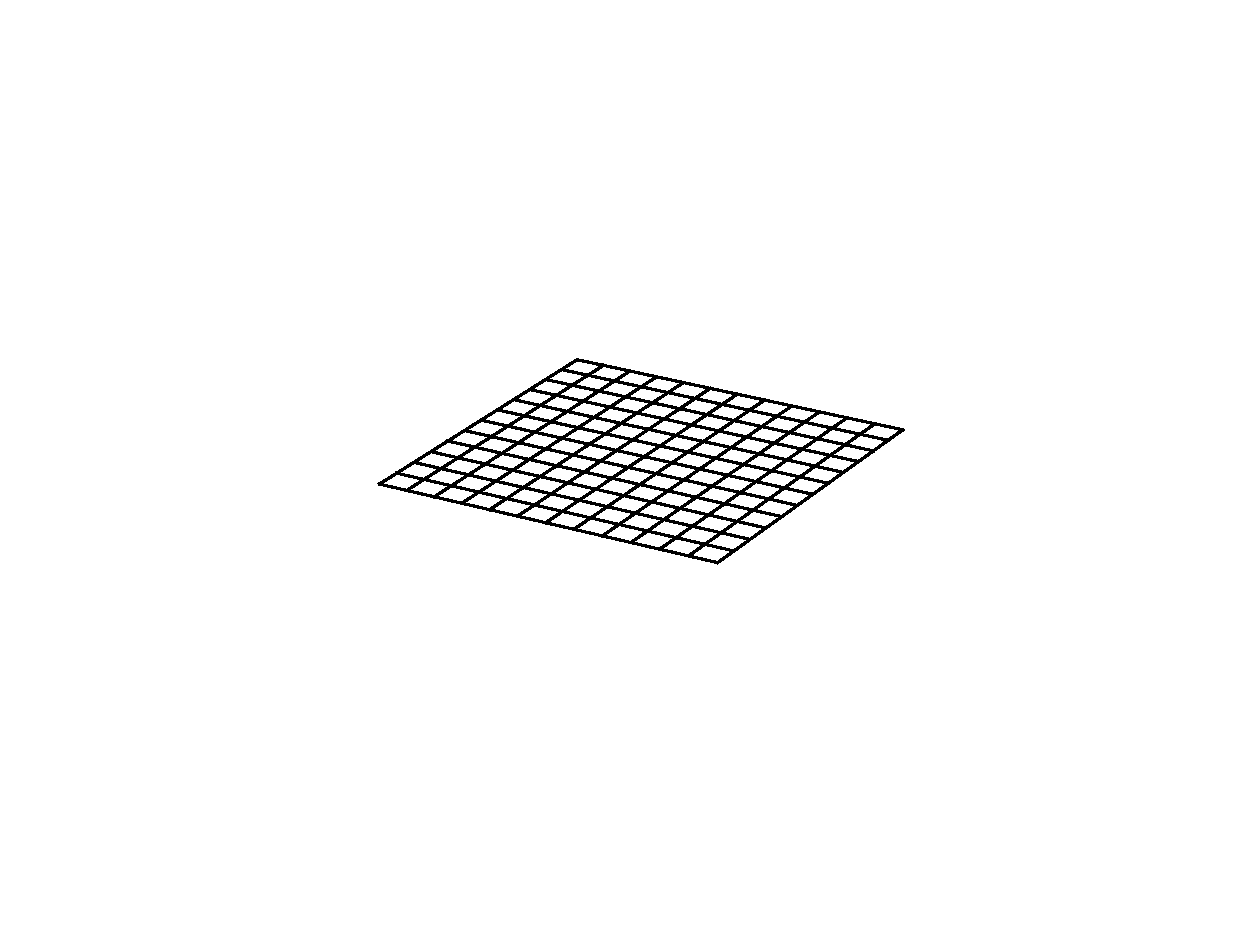
\includegraphics[trim=175 165 140 165, clip, scale=0.4]{../paper/FIG/tc1_platform}
                \end{figure}\end{textblock}
        }
        \only<2->{
            \begin{textblock}{9}(-1,1)\textbf{Problem:} Find best antenna placements to maximize gain and minimize coupling \end{textblock}
            \begin{textblock}{3}(2.5,1.5)
                \begin{figure}
                    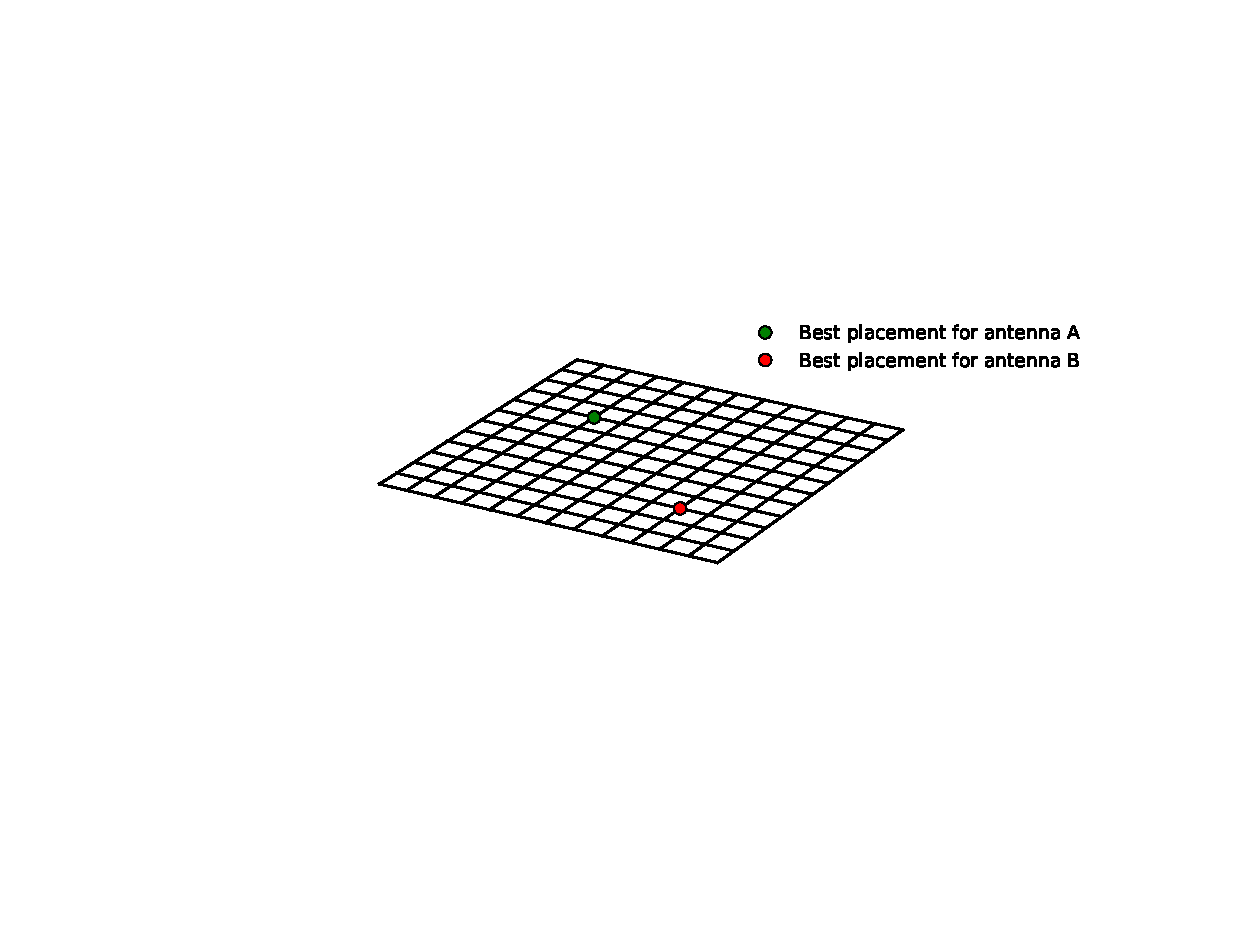
\includegraphics[trim=170 165 70 145, clip, scale=0.4]{../paper/FIG/tc11_intro}
                \end{figure}\end{textblock}
        }
        \column{0.33\linewidth}
        \only<1->{
            \begin{textblock}{6}(-1.5,-2.8) + \end{textblock}
            \begin{textblock}{6}(-0.7,-2.8) allowable placements of antennas \end{textblock}
            \begin{textblock}{3}(-0.2,-2)
                \begin{figure}
                    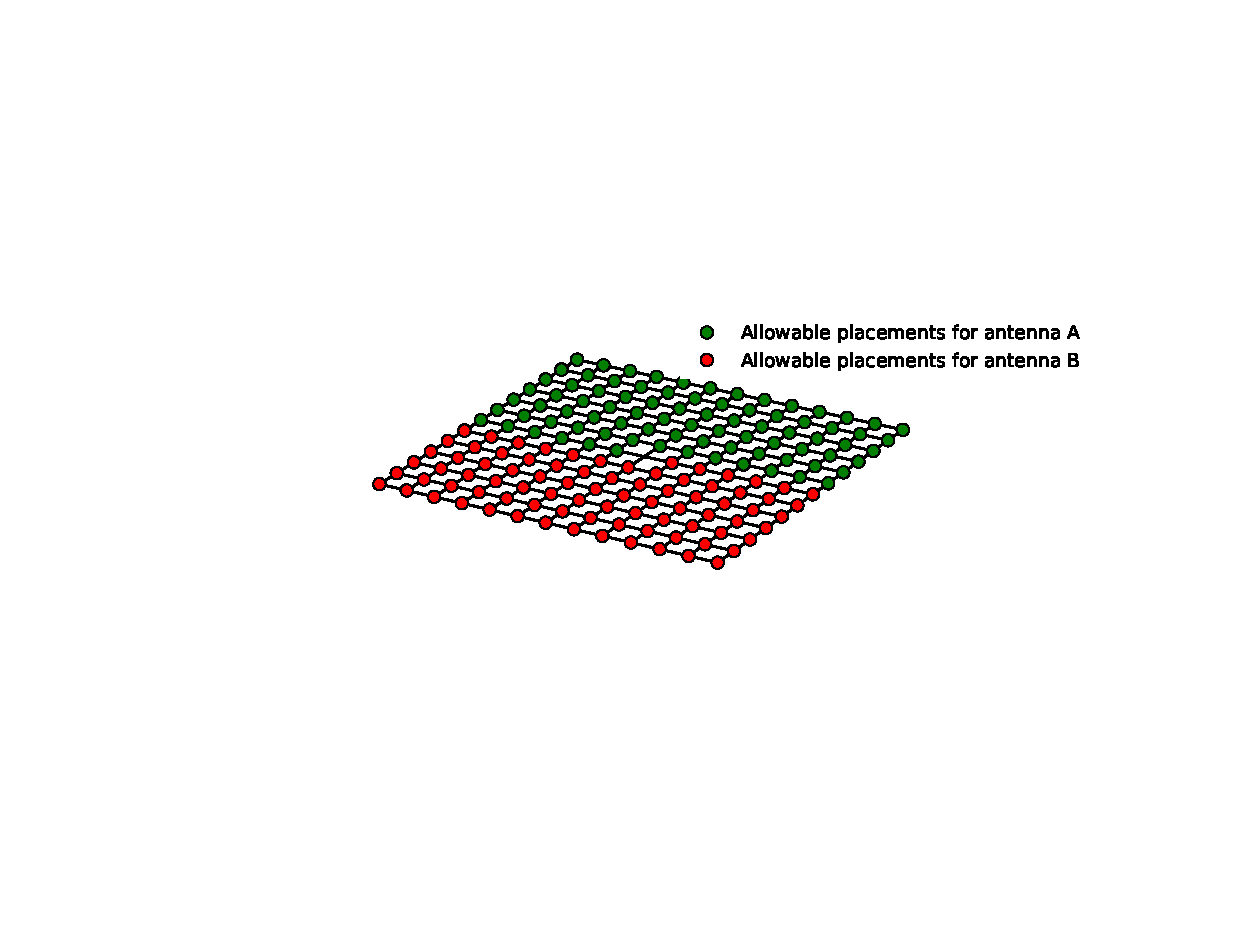
\includegraphics[trim=170 165 65 145, clip, scale=0.4]{../paper/FIG/tc1_intro}
                \end{figure}\end{textblock}
        }
    \end{columns}
\end{frame}

\begin{frame}[t]{Antenna Placement Problem}
    Given:
\begin{itemize} \itemsep1.5em
        \item platform $P$ with its surface gridded such that end points represent possible antenna placements
        \item set of  $n$ antennas $A = {A_1, A_2, \dots, A_n}$ such that $n > 1$
        \item for each $A_i$, $L_i$ denote the set of allowable placements $\in \mathbb R^3$ such that $\mid L_i \mid = m_i$ and $\forall i, m_i > 1$\[ L_i = \{(x_{1}, y_{1}, z_{1}) \dots (x_{m_i}, y_{m_i}, z_{m_i})\} \]
    \end{itemize}
    \textbf{Problem}: Find a set of $n$ optimal antenna placements on $P$ to maximize gain and minimize coupling. \\
    \vspace*{2mm}
    \textbf{Size of search space} $= \mathbf{m^n}$, if $m_i = m, \forall i \in [1,n]$
\end{frame}

\begin{frame}{\null}
    \begin{tcolorbox}[colback=green!5]
        \centering
        Question: How is a good antenna placement quantified in the context of platform and other antennas?
    \end{tcolorbox}
\end{frame}

\begin{frame}[t]{Mutual Coupling}
    When two antennas are in proximity, and one is transmitting, the second will receive some of the transmitted energy.\\ \vspace{2mm}
    \begin{figure}\centering
        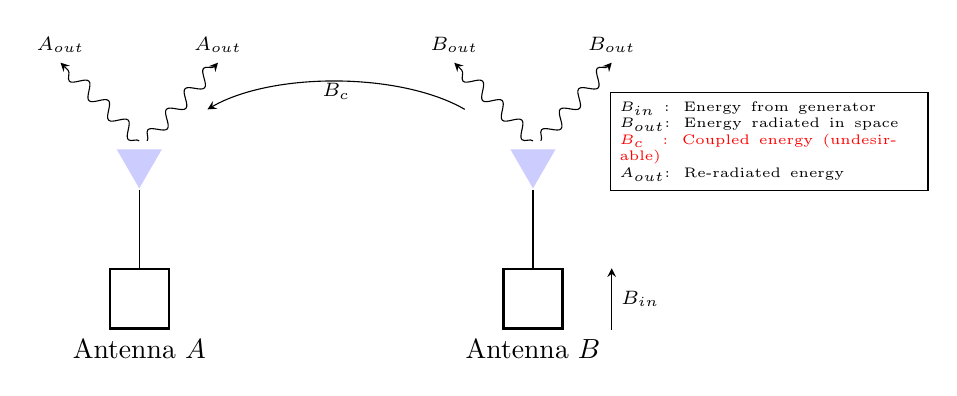
\begin{tikzpicture} [
                triangle/.style = {fill=blue!20, regular polygon, regular polygon sides=3 },
                node rotated/.style = {rotate=180},
                border rotated/.style = {shape border rotate=180}
            ]
            \node (b1) at (0, 1) [draw,thick,minimum width=.75cm,minimum height=.75cm, label=below:Antenna $A$] {}; 
            \node[triangle, border rotated, above=1cm of b1] (a1) {};
            \draw [-] (a1) -- (b1);
            \node (b2) at (5, 1) [draw,thick,minimum width=.75cm,minimum height=.75cm, label=below:Antenna $B$] {}; 
            \node[triangle, border rotated, above=1cm of b2] (a2) {};
            \draw [-] (a2) -- (b2);
            \draw [-stealth] ([xshift=1cm] b2.south) to node[right] {\scriptsize $B_{in}$} ([xshift=1cm] b2.north);
            \draw [stealth-, shorten <= 1cm, shorten >= 1cm] (a1.north) to[bend left] node {\scriptsize $B_c$} (a2.north);
            \draw [-stealth,decorate,decoration=snake] ([yshift=.1cm, xshift=.1cm] a1.north) -- (1,4) node[above] {\scriptsize $A_{out}$};
            \draw [-stealth,decorate,decoration=snake] ([yshift=.1cm] a1.north) -- (-1,4) node[above] {\scriptsize $A_{out}$};
            \draw [-stealth,decorate,decoration=snake] ([yshift=.1cm, xshift=.1cm] a2.north) -- (6,4) node[above] {\scriptsize $B_{out}$};
            \draw [-stealth,decorate,decoration=snake] ([yshift=.1cm] a2.north) -- (4,4) node[above] {\scriptsize $B_{out}$};
            \node[draw, text width=3.8cm] at (8,3) {\tiny $B_{in}~$:  Energy from generator\\$B_{out}$: Energy radiated in space\\{\color{red}$B_c~~$: Coupled energy (undesirable)}\\$A_{out}$: Re-radiated energy\\}; 
        \end{tikzpicture}
    \end{figure}
\end{frame}

\begin{frame}{Minimize Mutual Coupling}
    \begin{tcolorbox}[colback=green!5]
        \begin{equation}
            F_{MC} = \sum_{i=1}^{n-1}\sum_{j=i+1}^{n} CP(A_i, A_j),
        \end{equation}
    \end{tcolorbox}
    where
    \begin{itemize}
        \item $CP(\cdot, \cdot) \in \mathbb R$ is the coupling between two antennas, and computed using a simulator
        \item There will be $n \choose 2$ coupling terms 
    \end{itemize}
    \vspace{2mm}
    \small\textit{Example:} If $n=3$, then $F_{MC} = CP(A_1, A_2) + CP(A_1, A_3) + CP(A_2, A_3)$
\end{frame}

\begin{frame}{Free Space Radiation Pattern}
    \begin{columns}
        \begin{column}{0.5\linewidth}
            \begin{figure}
                \vspace{-2.5cm}
                \centering
                \includegraphics[width=4cm, height=5cm]{../paper/FIG/free_space.png}
                \caption*{\tiny Free-space patten without platform or other antennas}
            \end{figure}
        \end{column}
        \begin{column}{0.5\linewidth}
            \begin{overlayarea}{\textwidth}{\textheight}
            \begin{figure}
                \begin{subfigure}{\columnwidth}
                \centering
                \includegraphics[scale=0.3]{../paper/FIG/free_cross.png}
                \caption*{\tiny 2D view of the \textcolor{blue}{free-space gain pattern}}%
            \end{subfigure}\vspace*{2mm}
    \begin{tcolorbox}[colback=green!5]
        \centering
        This is ideal pattern since there is no interference
    \end{tcolorbox}
            \end{figure}
    \end{overlayarea}
        \end{column}
    \end{columns}
\end{frame}

\begin{frame}{Radiation Pattern}
    \begin{columns}
        \begin{column}{0.5\linewidth}
            \begin{figure}
                \vspace{-2.5cm}
                \centering
                \includegraphics[width=4cm, height=5cm]{../paper/FIG/free_space.png}
                \caption*{\tiny{Ideal gain pattern since there is no intereference}}
            \end{figure}
        \end{column}
        \begin{column}{0.5\linewidth}
            \begin{overlayarea}{\textwidth}{\textheight}
            \begin{figure}
                \begin{subfigure}{\columnwidth}
                \centering
                \includegraphics[scale=0.3]{../paper/FIG/free_cross.png}
                \caption*{\tiny {2D view of the \textcolor{blue}{free-space gain pattern}}}%
            \end{subfigure}\vspace*{2mm}
            \begin{subfigure}{\columnwidth}
                \centering
                \includegraphics[scale=0.3]{../paper/FIG/comp_cross.png}
                \caption*{\tiny {\textcolor{red}{In-situ gain pattern} for random antenna placements different from \textcolor{blue}{free-space gain pattern}}}%
            \end{subfigure}
            \end{figure}
    \end{overlayarea}
        \end{column}
    \end{columns}
\end{frame}



\begin{frame}{Minimize Difference in Radiation Pattern}
    \begin{tcolorbox}[colback=green!5]
        \begin{equation} \label{eq:rp}
            F_{RP} = \sum_{i=1}^n~\sum_{\theta=0}^{\frac{180\degree}{S}}~\sum_{\phi=0}^{\frac{360\degree}{S}}
            \left( FSG_i(S\theta,S\phi) - ISG_i(S\theta,S\phi) \right) ^2,
        \end{equation}
    \end{tcolorbox}
    where
    \begin{itemize}
            \small
        \item $S$ is the step size
        \item $\theta, \phi$ spherical coordinates in degrees
        \item $FSG(\cdot,\cdot) \in \mathbb R$ is the free-space gain pattern computed by the simulator
        \item $ISG(\cdot,\cdot) \in \mathbb R$ is the in-situ gain pattern computed by the simulator
    \end{itemize}
\end{frame}

\begin{frame}{Fitness Evaluation}
    Find a placement such that $F$ is minimal:
    \begin{tcolorbox}[colback=green!5]
        \begin{equation} \label{eq:optimal}
            F = \alpha F_{MC} + \beta F_{RP},
        \end{equation}
    \end{tcolorbox}
    where $\alpha, \beta$ are adjustable weights for each of the objectives 
\end{frame}

\begin{frame}{\null}
    \begin{tcolorbox}[colback=green!5]
        \centering\Huge
        Part 2: Stochastic Algorithms
    \end{tcolorbox}
\end{frame}
\begin{frame}{\null}
    \begin{tcolorbox}[colback=green!5]
        \centering
        Question: Why use stochastic algorithms?
    \end{tcolorbox}
\end{frame}

\begin{frame}[t]{Multi-Modal Search Space}
    \begin{figure}
        \vspace*{-0.35cm}
        \centering
        \includegraphics[scale=0.4]{../paper/FIG/tc1_ss}
        \caption*{Search space for one of the test cases evaluated. There are multiple local minimas which makes convergence difficult. z-axis is the combined fitness $F$}
    \end{figure}
\end{frame}


\begin{frame}[t]{Stochastic Algorithms}
    We will consider algorithms which are based on randomization principle.
    \vspace{10px}
\begin{itemize} \itemsep1.5em
        \item Genetic Algorithm
        \item Evolutionary Strategy
        \item Simulated Annealing
        \item Hill Climbing
    \end{itemize}
    \vspace{5mm}
    Each algorithm maintains a candidate solution or pool of candidate solutions called population
\end{frame}

\begin{frame}[t]{Stochastic Algorithms: Operand}
    \textbf{Candidate solution} or an \textbf{individual} is a member of a set of possible solutions.
\begin{itemize} \itemsep1.5em
               \item Simulated Annealing and Hill Climbing maintain single individual\\
            \adjustbox{valign=t}{%
                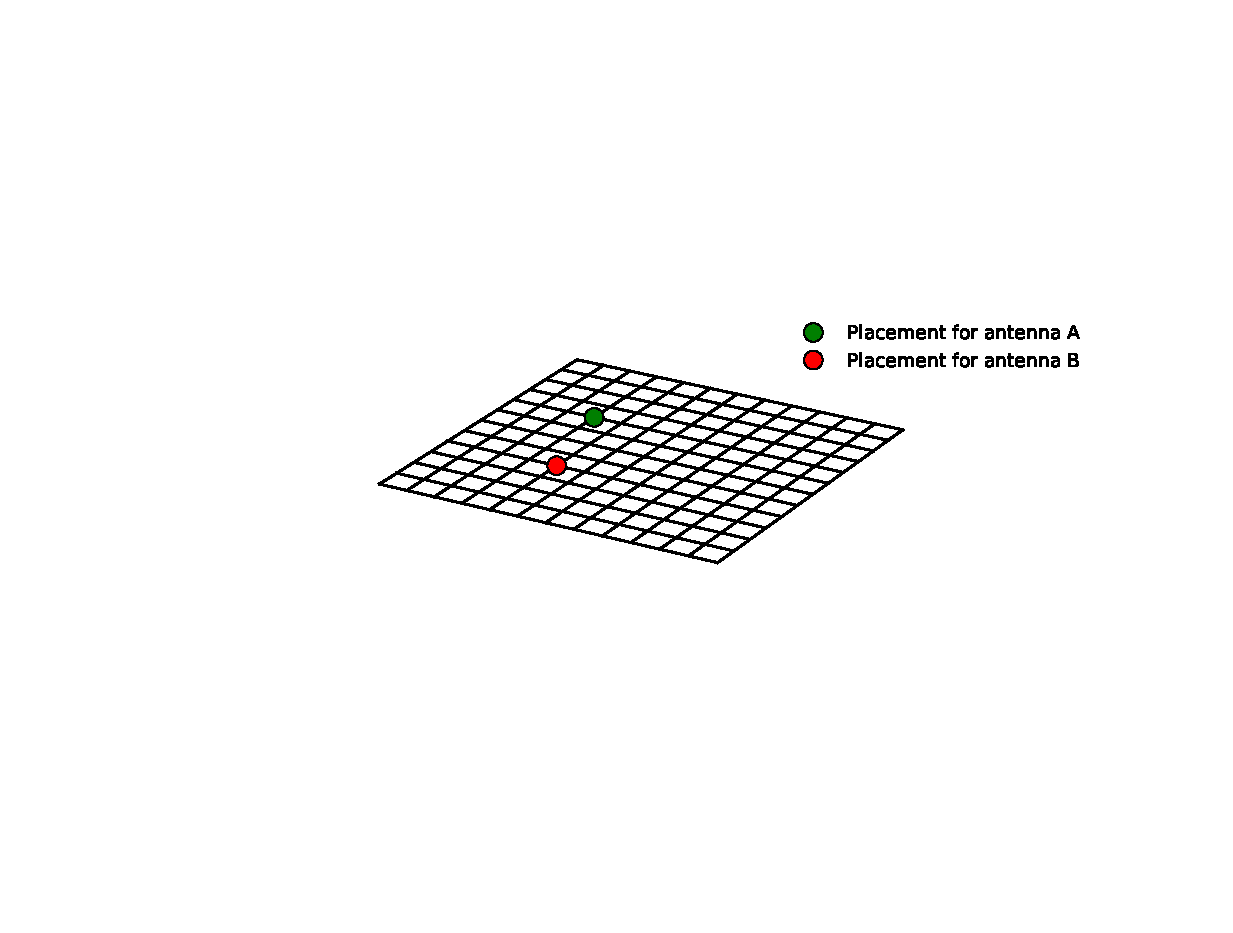
\includegraphics[trim=125 165 50 135, clip, scale=0.35]{../paper/FIG/tc1_mut3}
            }
    \item Genetic Algorithm and Evolutionary Strategy maintain a population of individuals
            \adjustbox{valign=t}{%
                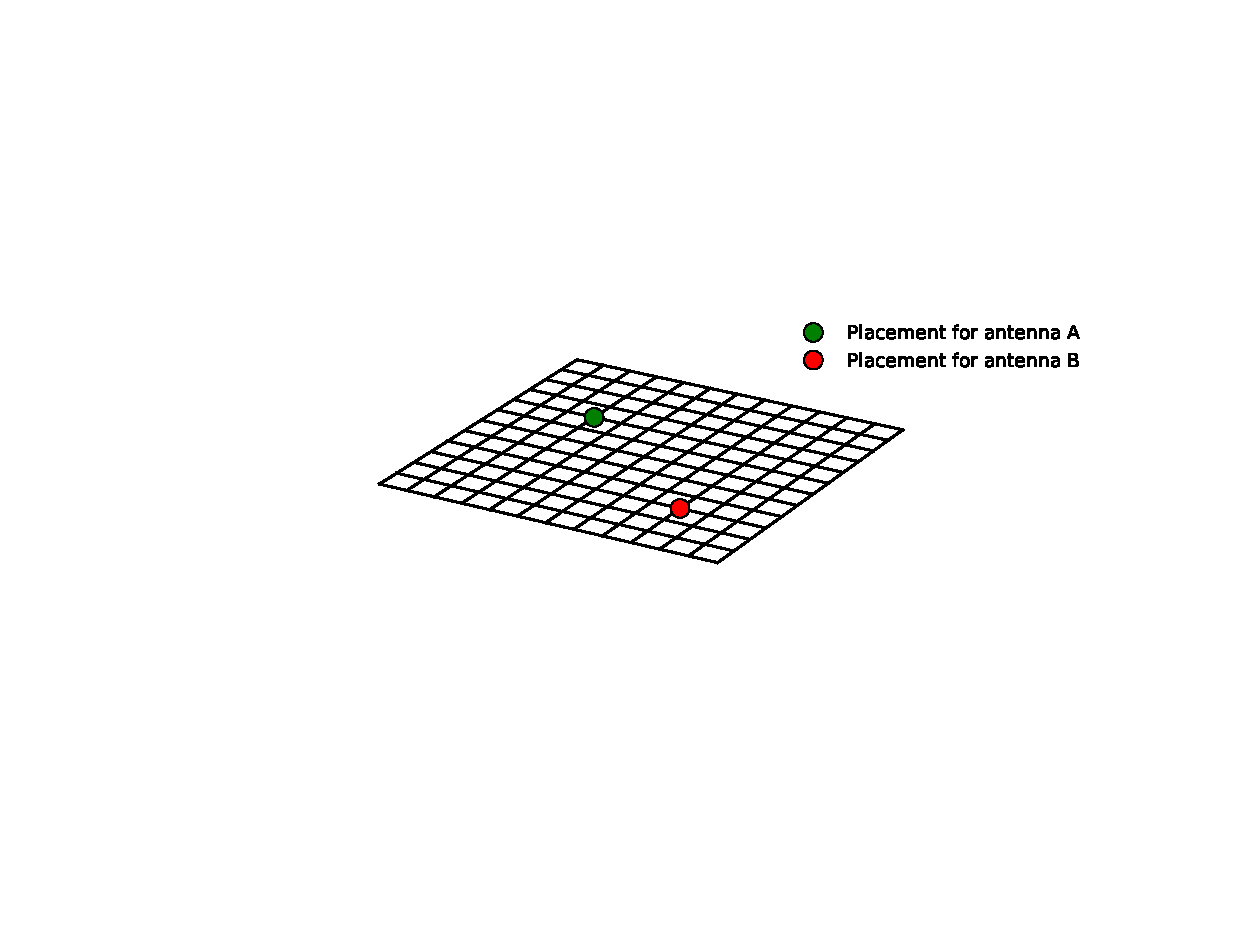
\includegraphics[trim=175 165 50 135, clip, scale=0.35]{../paper/FIG/tc1_mut1}
                $\bigcdot~\bigcdot~\bigcdot$
                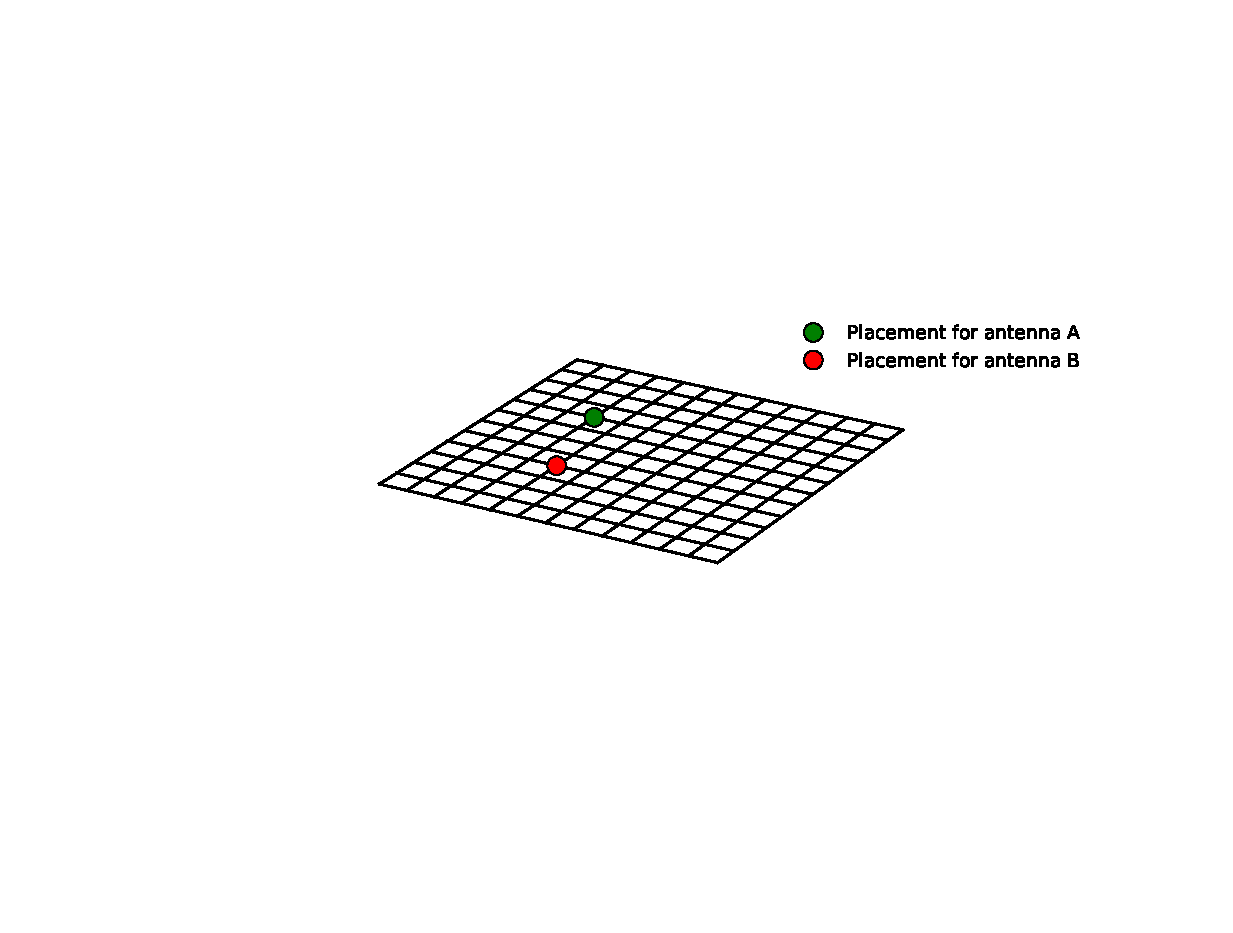
\includegraphics[trim=125 165 50 135, clip, scale=0.35]{../paper/FIG/tc1_mut3}
            }
    \end{itemize}
\end{frame}

\begin{frame}[t]{Stochastic Algorithms: Mutation Operator}
    \begin{enumerate}
        \item Given an individual, select an antenna uniformly at random, let's say antenna 1:\par
            \begin{minipage}[t]{\linewidth}
                \centering
                \adjustbox{valign=t}{%
                    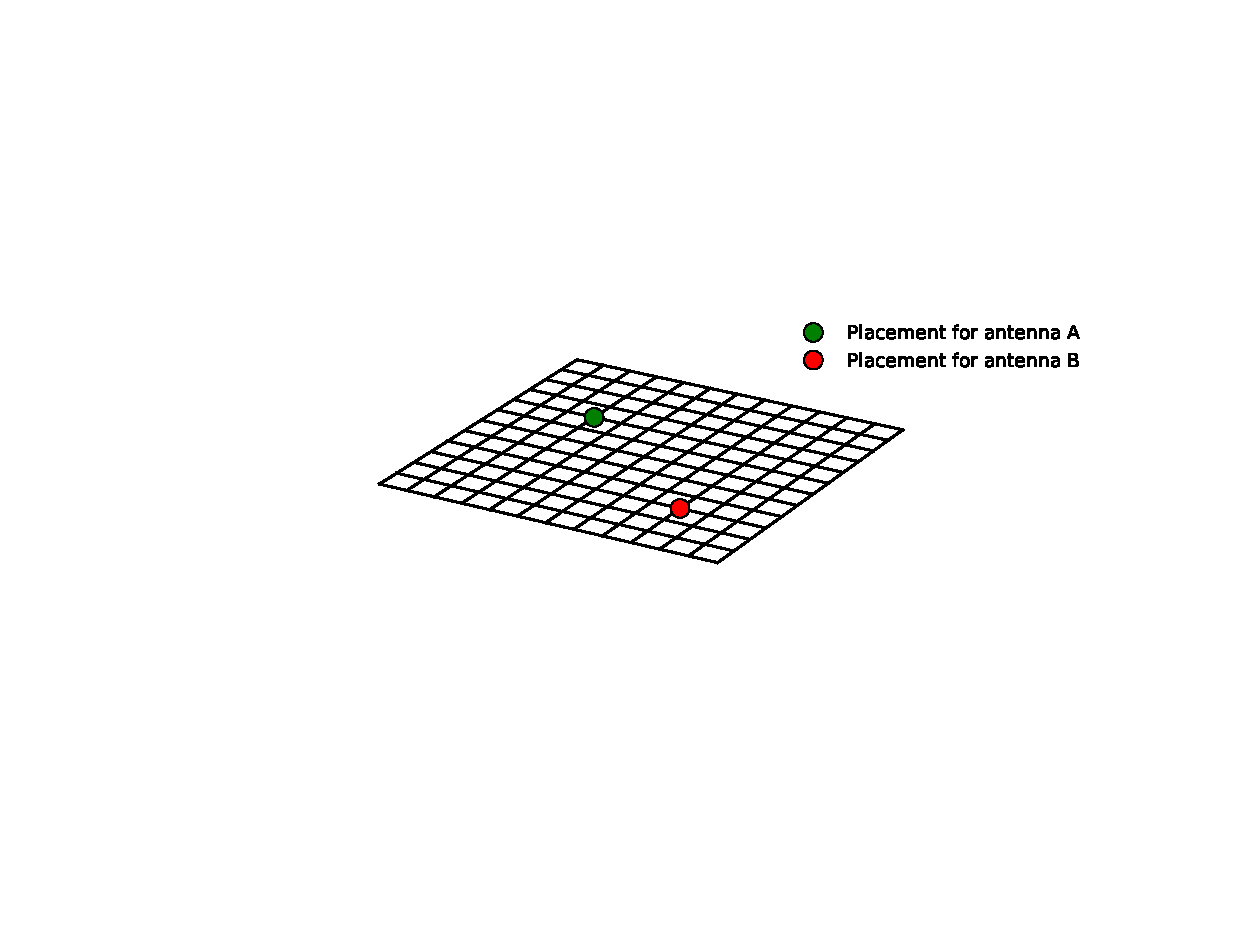
\includegraphics[trim=175 165 50 135, clip, scale=0.35]{../paper/FIG/tc1_mut1}
                }
            \end{minipage}
        \item For antenna 1, select any other allowable placement:\par
            \begin{minipage}[t]{\linewidth}
                \centering
                \adjustbox{valign=t}{%
                    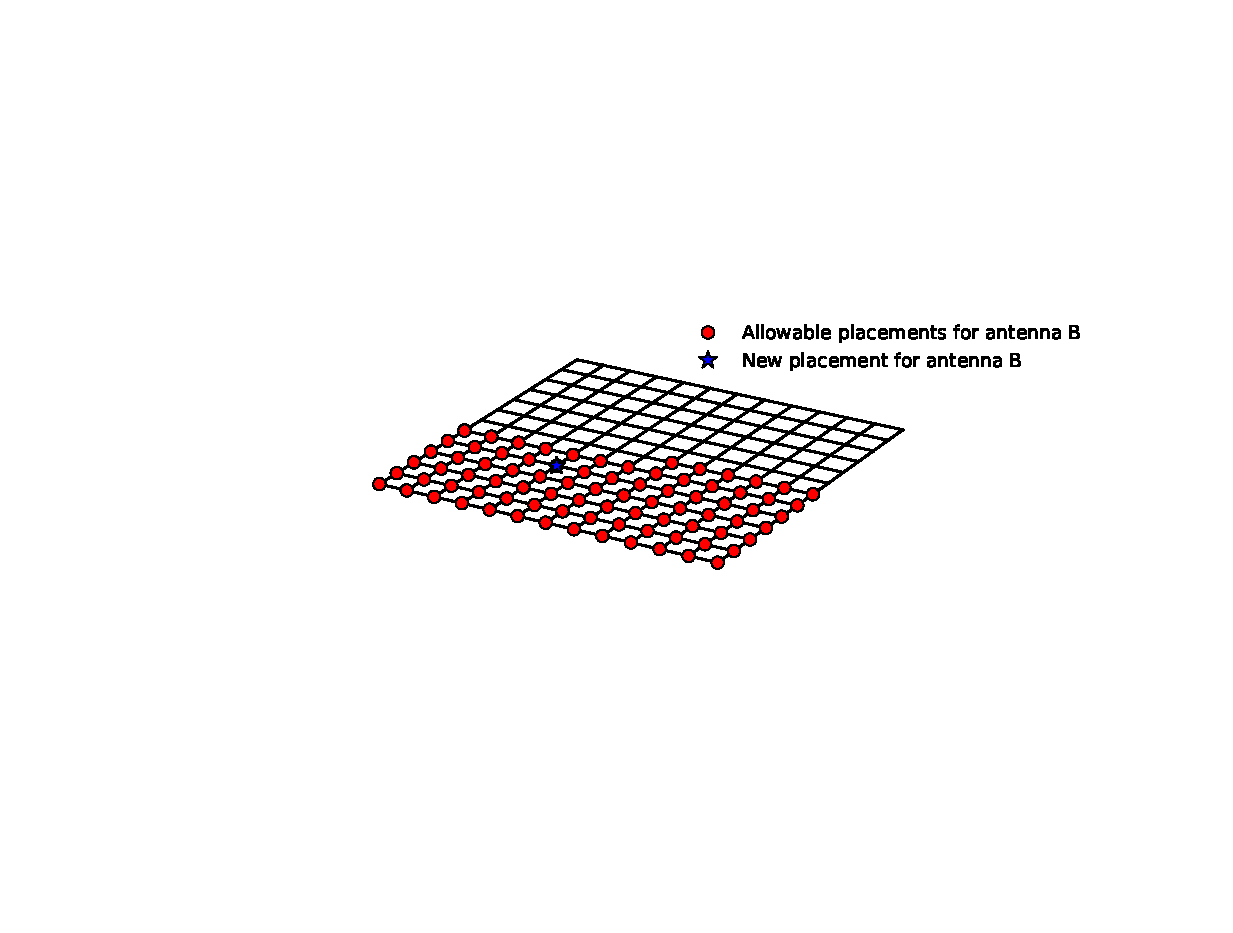
\includegraphics[trim=125 165 50 135, clip, scale=0.35]{../paper/FIG/tc1_mut2}
                }
            \end{minipage}
        \item Change position for antenna 1 in individual:\par
            \begin{minipage}[t]{\linewidth}
                \centering
                \adjustbox{valign=t}{%
                    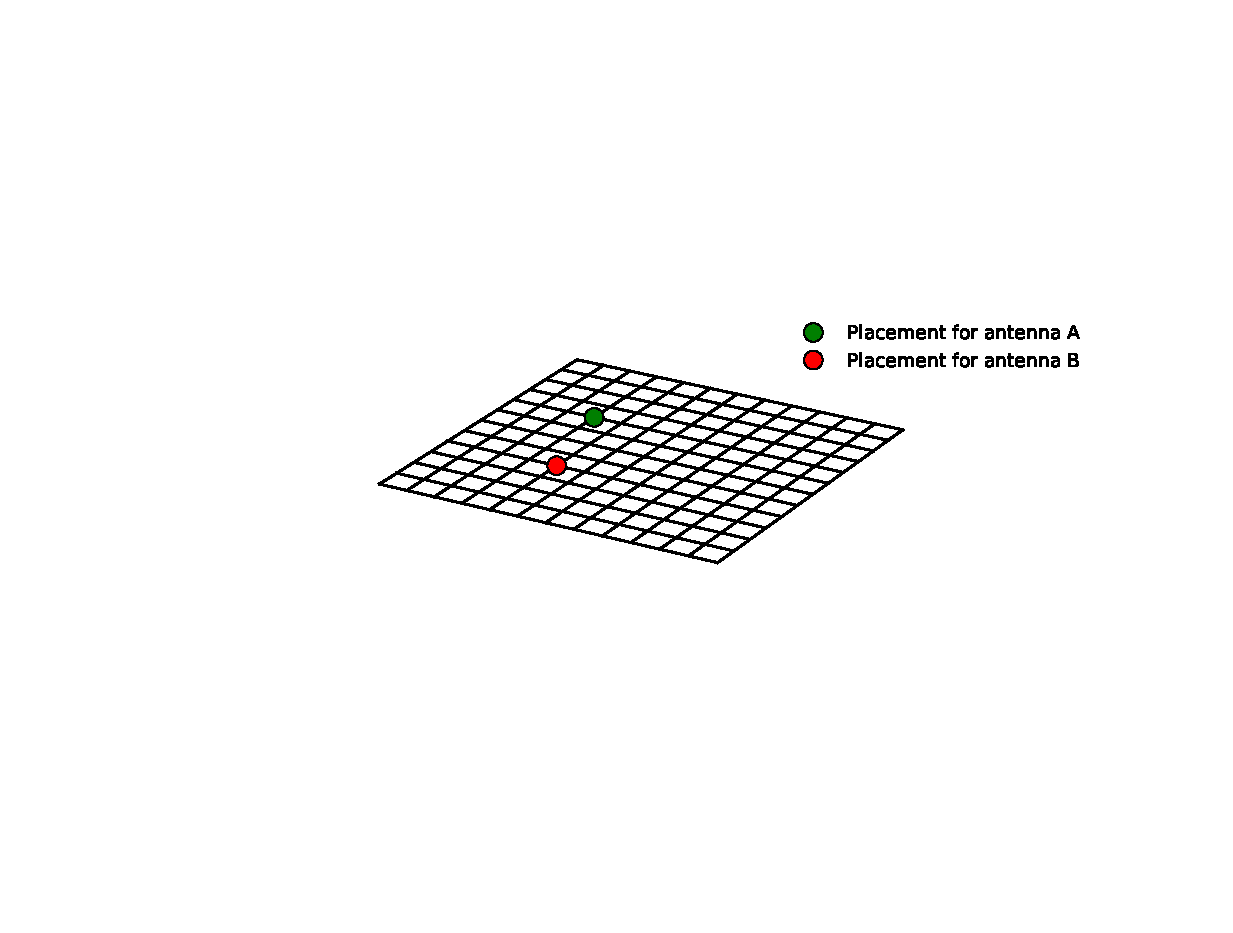
\includegraphics[trim=125 165 50 135, clip, scale=0.35]{../paper/FIG/tc1_mut3}
                }
            \end{minipage}
    \end{enumerate}
\end{frame}

\begin{frame}[t]{Stochastic Algorithms: Crossover Operator}
    \begin{enumerate}
        \item Select two individuals from population:\par
            \begin{minipage}[t]{\linewidth}
                \centering
                \adjustbox{valign=t}{%
                    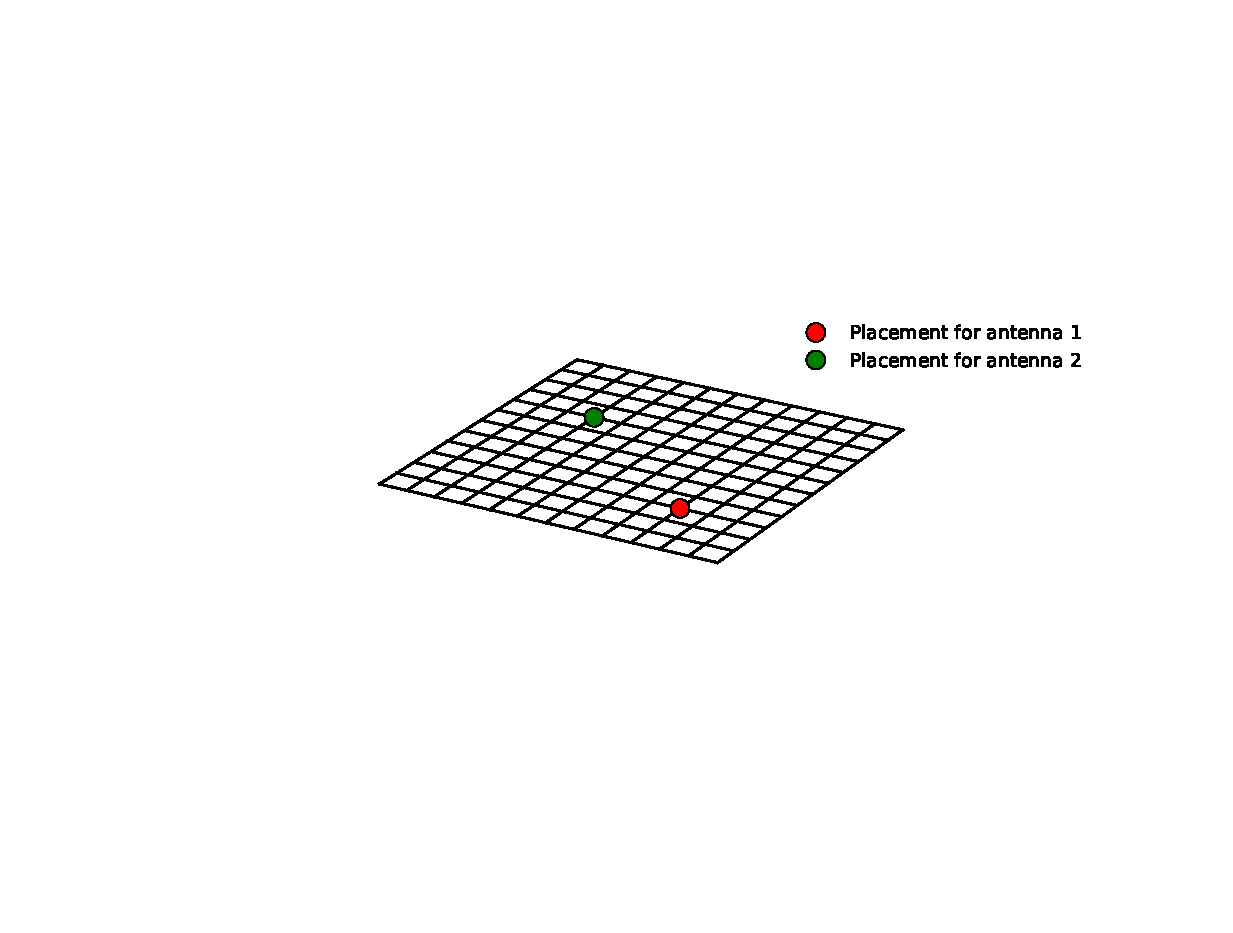
\includegraphics[trim=175 165 50 135, clip, scale=0.35]{../paper/FIG/tc1_reco1}
                    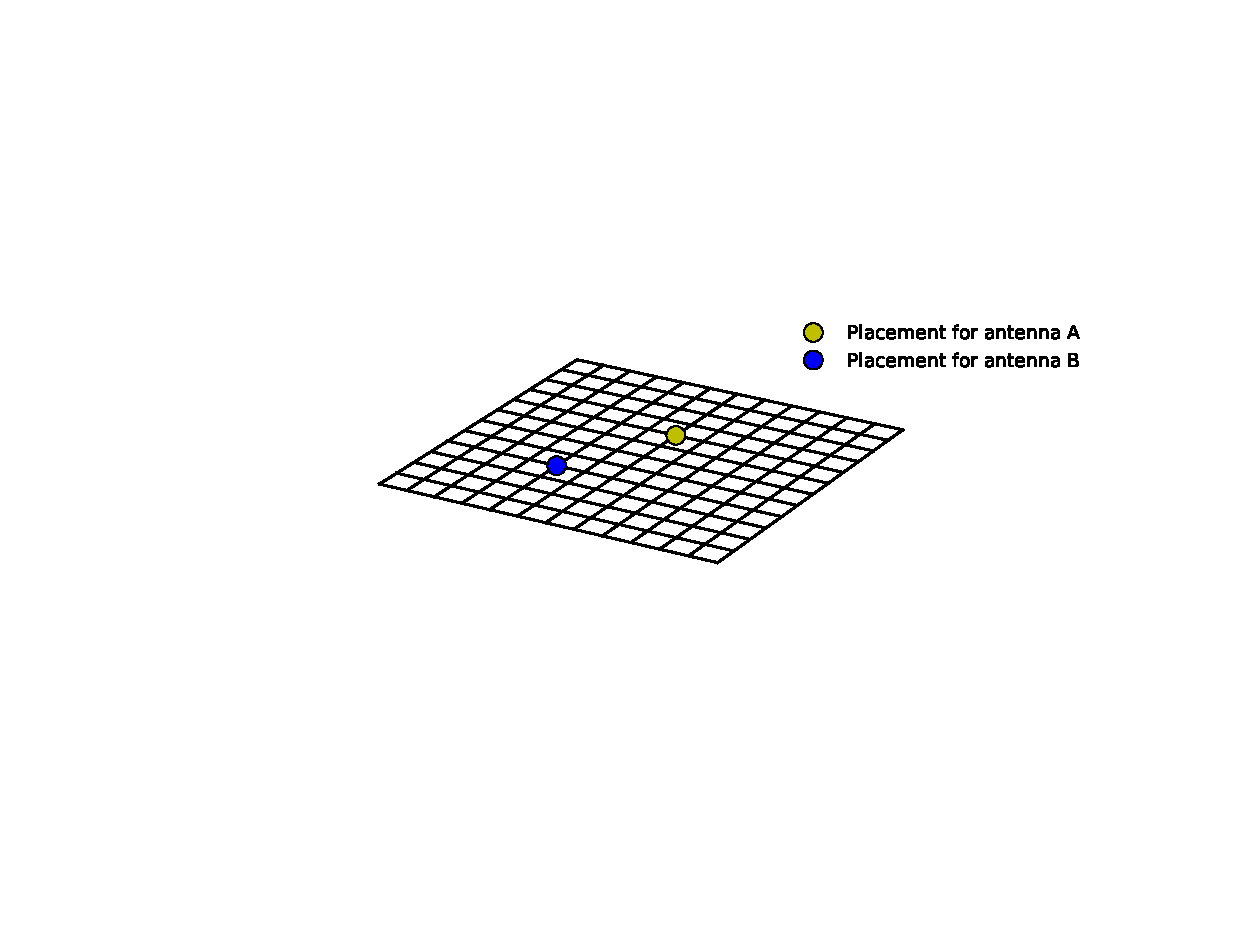
\includegraphics[trim=175 165 50 135, clip, scale=0.35]{../paper/FIG/tc1_reco2}
                }
            \end{minipage}
        \item Select a crossover point, and swap placements prior to the point: \par
            \begin{minipage}[t]{\linewidth}
                \centering
                \adjustbox{valign=t}{%
                    \begin{tabular}{ll:l}
                        $\text{ind}_1:$&$\textcolor{red}{A_1}$ & $\textcolor{drkgreen}{A_2}$ \\
                        &\makebox[\widthof{A\_1}][l]{$\downarrow~\uparrow$} &\\
                        $\text{ind}_2:$&$\textcolor{blue}{A_1}$ & $\textcolor{aureolin}{A_2}$ \\
                    \end{tabular}
                }
            \end{minipage}
        \item Two new offsprings created:\par
            \begin{minipage}[t]{\linewidth}
                \centering
                \adjustbox{valign=t}{%
                    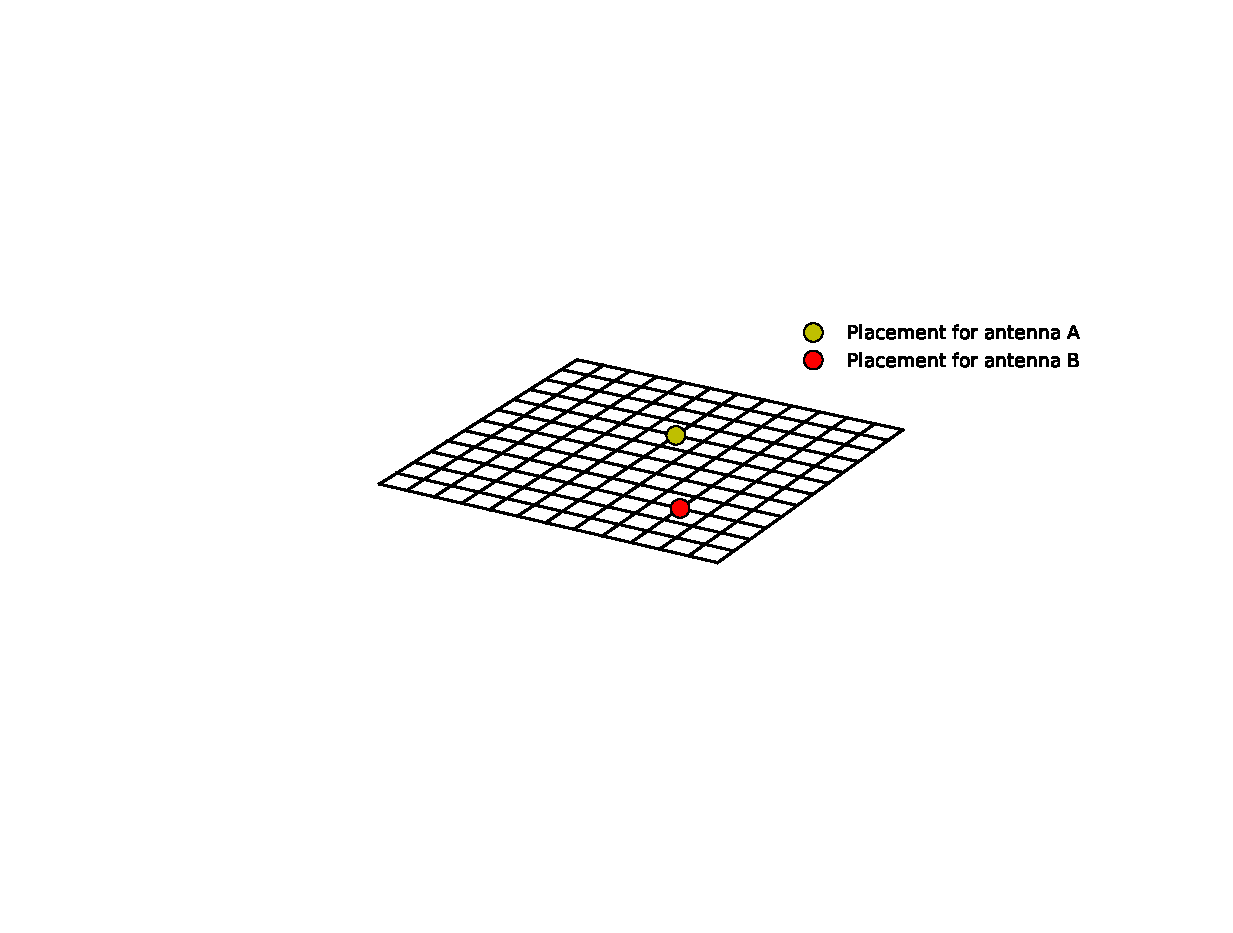
\includegraphics[trim=175 165 50 135, clip, scale=0.35]{../paper/FIG/tc1_reco3}
                    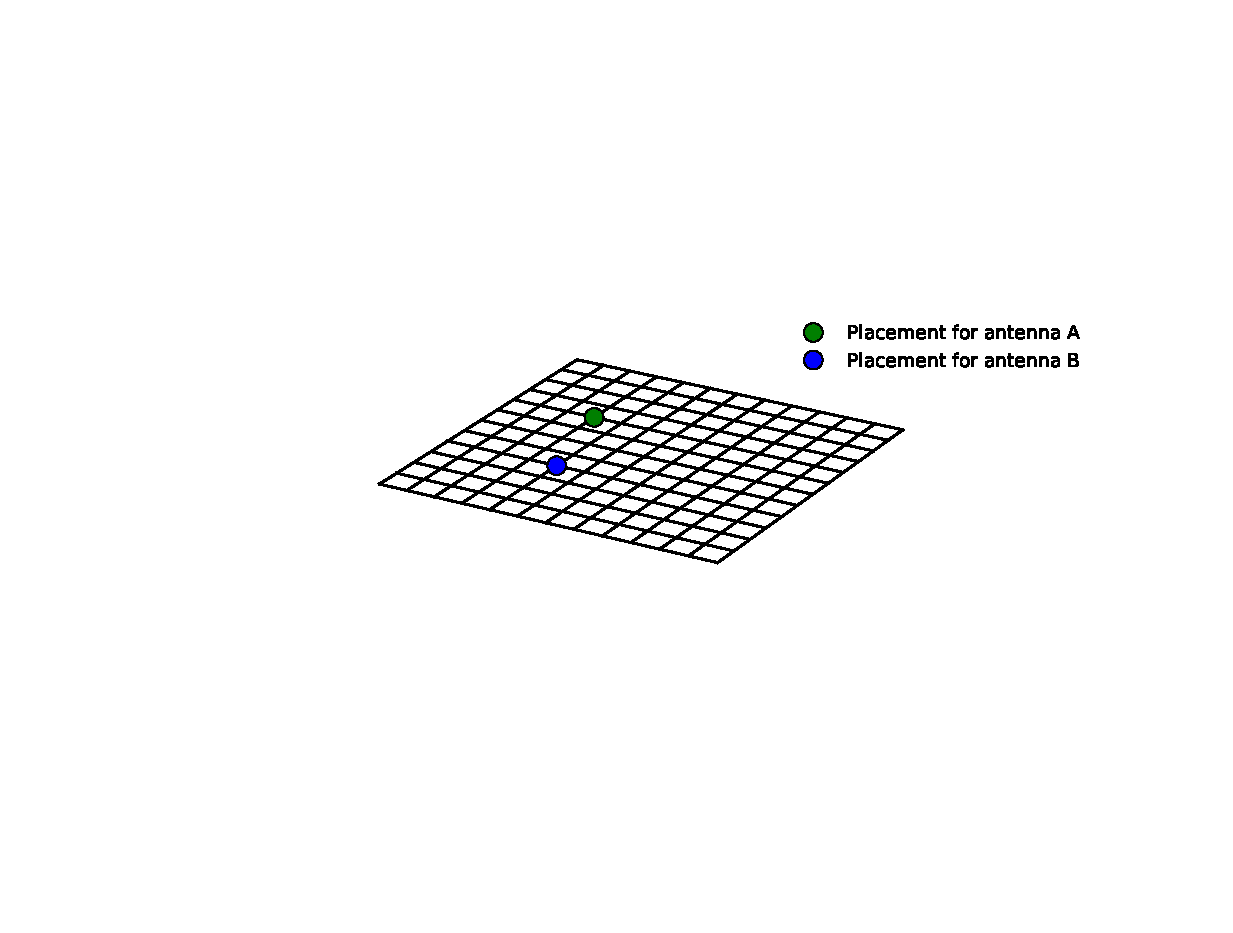
\includegraphics[trim=175 165 50 135, clip, scale=0.35]{../paper/FIG/tc1_reco4}
                }
            \end{minipage}
    \end{enumerate}
\end{frame}

\begin{frame}{Genetic Algorithm}
    \begin{columns}
        \begin{column}{0.66\linewidth}%added for this algorithm since text wasn't fitting in one slide
            \begin{spacing}{0.6}
                \fontsize{8}{12}\selectfont
                \setlength{\interspacetitleruled}{0pt}%
                \setlength{\algotitleheightrule}{0pt}%
                \begin{algorithm}[H]
                    \only<1>{\reduline{\textbf{P} $\leftarrow$ generate $p$ random individuals. Compute $fitness(\textbf{ind}_i), i \in [1,p]$}\;}
                    \only<2>{\textbf{P} $\leftarrow$ generate $p$ random individuals. Compute $fitness(\textbf{ind}_i), i \in [1,p]$\;}
                    $i=0$ \;
                    \While{$i<gen_{max}$} {
                        \only<1>{Elitism: Select $n_e$ fittest individuals to add to \textbf{P'} \;}
                        \only<2>{\reduline{Elitism: Select $n_e$ fittest individuals to add to \textbf{P'}} \;}
                        \For{$(p - n_e)/2$ times} {
                            {\tiny \tcc{'select' returns a pair of individuals}}
                            $\textbf{M} \leftarrow select(\textbf{P}, 2)$  \;
                            \eIf {$rand(0,1)<p_c$} {
                                \only<1>{\textbf{O} $\leftarrow crossover(\textbf{M})$ \;}
                                \only<2>{\reduline{\textbf{O} $\leftarrow crossover(\textbf{M})$} \;}
                                Add $O$ to $P'$ \;
                            }
                            { Add $M$ to $P'$ \; }
                        }
                        \only<1>{Uniformly select $p_{m} \cdot (p - n_e)$ individuals from $P$, and apply $mutation$ operator to each \;}
                        \only<2>{\reduline{Uniformly select $p_{m} \cdot (p - n_e)$ individuals from $P$, and apply $mutation$ operator to each} \;}
                        Update $P\leftarrow P'$ \;
                        Compute $fitness(\textbf{ind}_i); i \in [1, p]$\;
                        Update $i \leftarrow i + 1$ \;
                    }
                \end{algorithm}
            \end{spacing}
        \end{column}
        \begin{column}{0.3\linewidth}
            \only<2->
            {
                \begin{figure}
                    \centerline{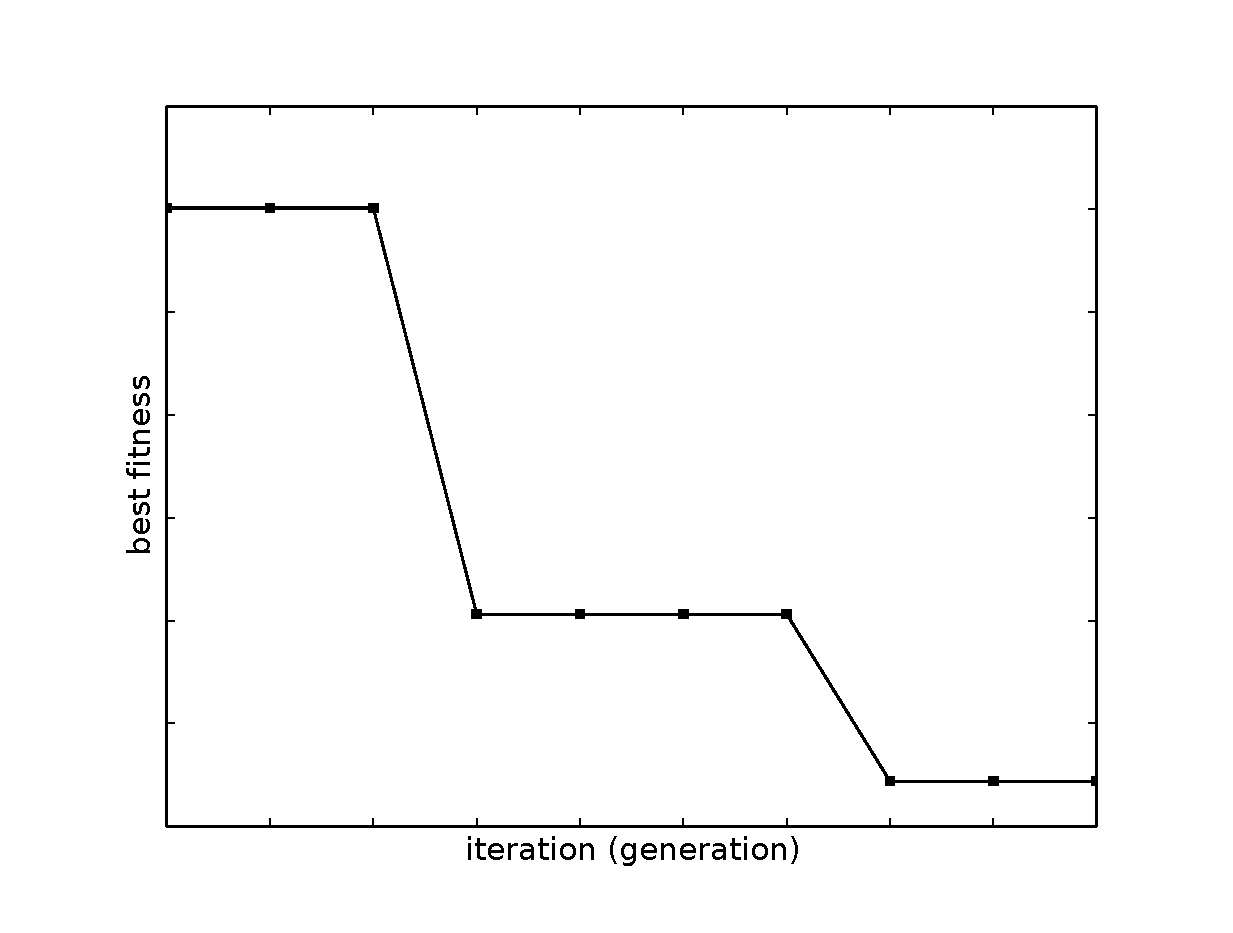
\includegraphics[width=5cm]{../paper/FIG/algo_ga}}
                    \caption*{Plateaus suggesting stagnation of search}
                \end{figure}
            }
        \end{column}
    \end{columns}
\end{frame}


\begin{frame}{Evolutionary Strategy}
    \begin{columns}
        \begin{column}{0.66\linewidth}
            \fontsize{8}{12}\selectfont
            \setlength{\interspacetitleruled}{0pt}%
            \setlength{\algotitleheightrule}{0pt}%
            \begin{algorithm}[H]
                \only<1>{\reduline{\textbf{P}$\leftarrow$ generate $\mu$ random individuals} \;}
                \only<2>{\textbf{P}$\leftarrow$ generate $\mu$ random individuals \;}
                $i=0$ \;
                \While{$i<gen_{max}$} {
                    \only<1>{Create $\lambda / \mu$ offsprings from  each $\mu$ individuals by applying $mutation$ operator\;}
                    Add all offsprings to \textbf{P} \;
                    \only<2>{\reduline{Create $\lambda / \mu$ offsprings from  each $\mu$ individuals by applying $mutation$ operator} \;}
                    Compute $fitness(\textbf{ind}_i), i \in [1,\lambda + \mu]$ \;
                    \only<1>{Keep $\mu$ best individuals in \textbf{P}, and discard remaining $\lambda - \mu$ individuals \;}
                    \only<2>{\reduline{Keep $\mu$ best individuals in \textbf{P}, and discard remaining $\lambda - \mu$ individuals} \;}
                    Update $i \leftarrow i+1$
                }
            \end{algorithm}
        \end{column}
        \begin{column}{0.3\linewidth}
            \only<2->
            {
                \begin{figure}
                    \centerline{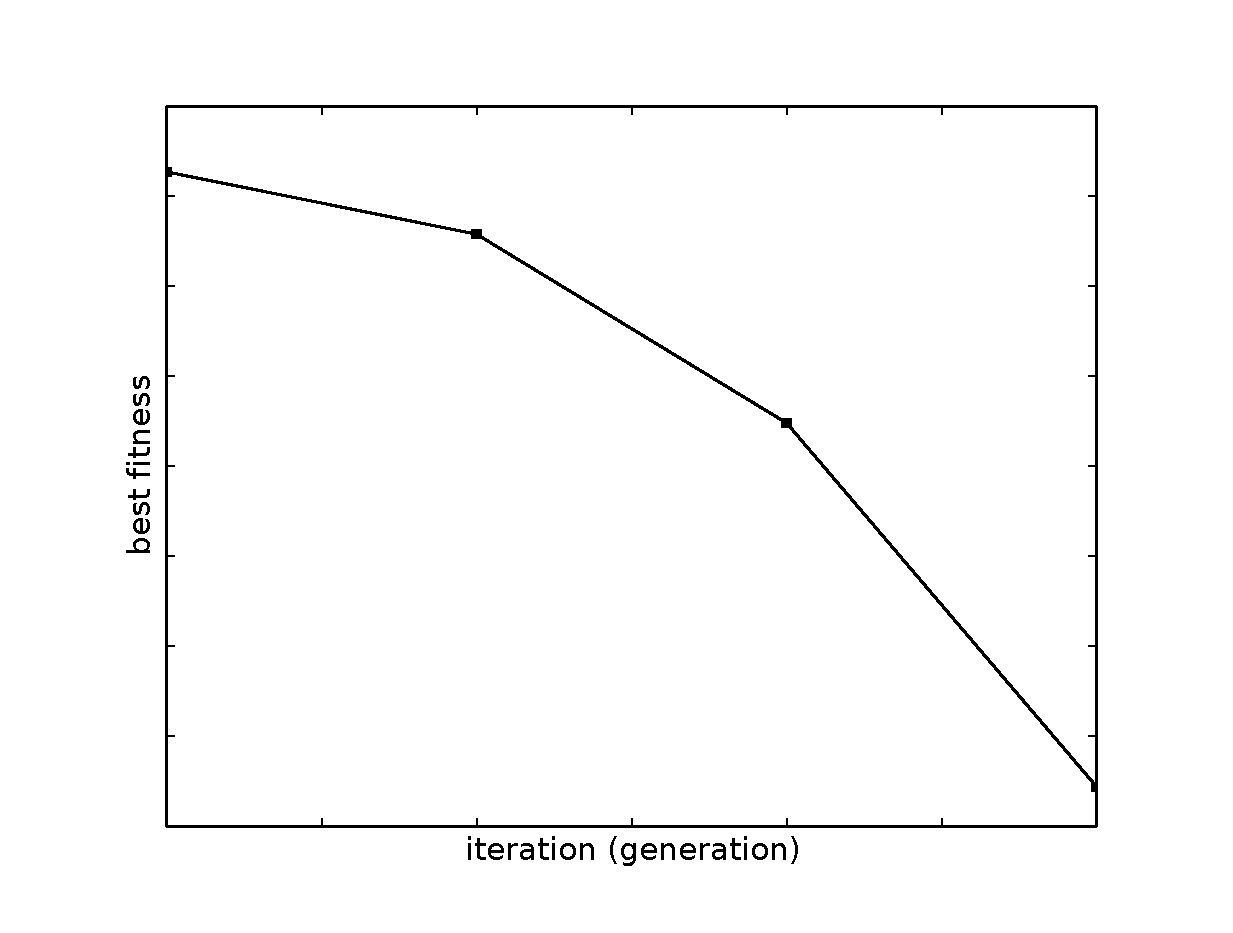
\includegraphics[width=5cm]{../paper/FIG/algo_es}}
                    \caption*{More mutations allow in-depth exploration of search space, and also makes rapid progress}
                \end{figure}
            }
        \end{column}
    \end{columns}
\end{frame}

\begin{frame}{Simulated Annealing}
    \begin{columns}
        \begin{column}{0.66\linewidth}
            \setlength{\interspacetitleruled}{0pt}%
            \setlength{\algotitleheightrule}{0pt}%
            \fontsize{8}{8}\selectfont
            \begin{algorithm}[H]
%\scriptsize
                \only<1>{\reduline{\textbf{c} $\leftarrow$ generate a random individual} \;}
                \only<2>{\textbf{c} $\leftarrow$ generate a random individual \;}
                $i=0$ \;
                \While{$i<i_max$} 
                {
                    \textbf{n} $\leftarrow mutate(\textbf{c})$ \; 
                    \eIf{$fitness(\textbf{c}) < fitness(\textbf{n})$} 
                    {
                        \If{\only<1>{$rand(0,1) < e^{-\delta f / T}$} \only<2>{\reduline{$rand(0,1) < e^{-\delta f / T}$}}} 
                        {
                            {\tiny \tcc{replace current individual by a higher fitness (less fitter) individual}}
                            \only<1>{\textbf{c} $ \leftarrow $ \textbf{n}}
                            \only<2>{\reduline{\textbf{c} $ \leftarrow $ \textbf{n}}}
                        }
                    }  {$\textbf{c} \leftarrow \textbf{n}$ \; }
                    \only<1>{$T \leftarrow T \cdot f_{cooling}$ \;}
                    \only<2>{\reduline{$T \leftarrow T \cdot f_{cooling}$} \;}
                    $i \leftarrow i + 1$ \;
                } 
                \label{alg:ap-sa}
            \end{algorithm}
        \end{column}
        \begin{column}{0.3\linewidth}
            \only<2->
            {
                \begin{figure}
                    \centerline{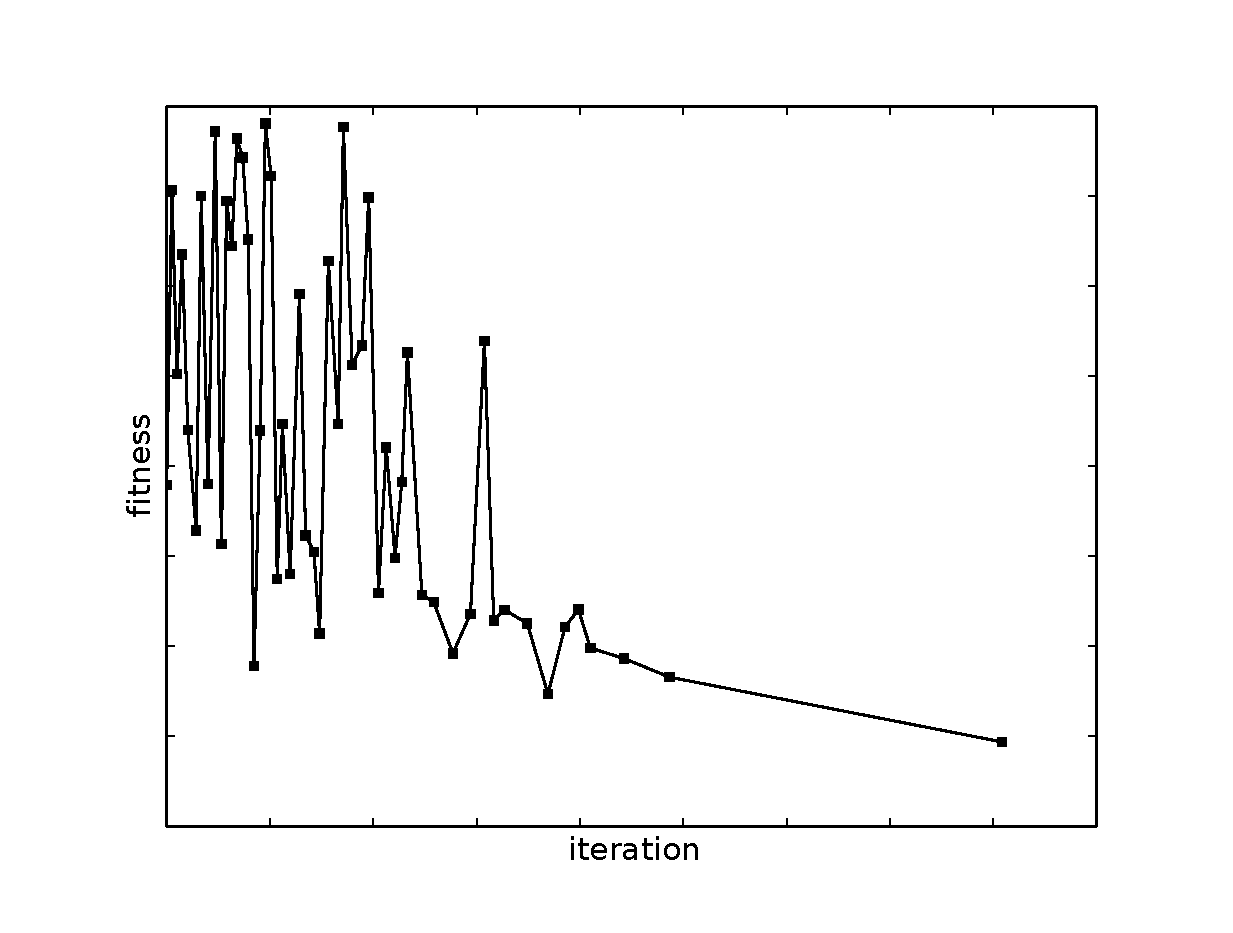
\includegraphics[width=5cm]{../paper/FIG/algo_sa}}
                    \caption*{Fluctuation in fitness gradually reduces due to cooling}
                \end{figure}
            }
        \end{column}
    \end{columns}
\end{frame}

\begin{frame}{Hill Climbing}
    \begin{columns}
        \begin{column}{0.66\linewidth}
            \setlength{\interspacetitleruled}{0pt}%
            \setlength{\algotitleheightrule}{0pt}%
            \fontsize{8}{8}\selectfont
            \begin{algorithm}[H]
                \only<1>{\reduline{Initialize \textbf{c} $\leftarrow$ generate a random inidividual} \;}
                \only<2>{Initialize \textbf{c} $\leftarrow$ generate a random inidividual \;}
                Compute $fitness(\textbf{c})$  \;
                $i=0$ \;
                \While{$i<i_{max}$} 
                {
                    \textbf{n} $\leftarrow mutate(\textbf{c})$ \; 
                    \If{\only<1>{$fitness(\textbf{n}) < fitness(\textbf{c})$} \only<2>{\reduline{$fitness(n) < fitness(c)$}}} 
                    {
                        \only<1>{$\textbf{c} \leftarrow \textbf{n}$} 
                        \only<2>{\reduline{$\textbf{c} \leftarrow \textbf{n}$}}
                    }
                    $i \leftarrow i + 1$
                }
                \label{alg:ap-hc}
            \end{algorithm}
        \end{column}
        \begin{column}{0.3\linewidth}
            \only<2->
            {
                \begin{figure}
                    \centerline{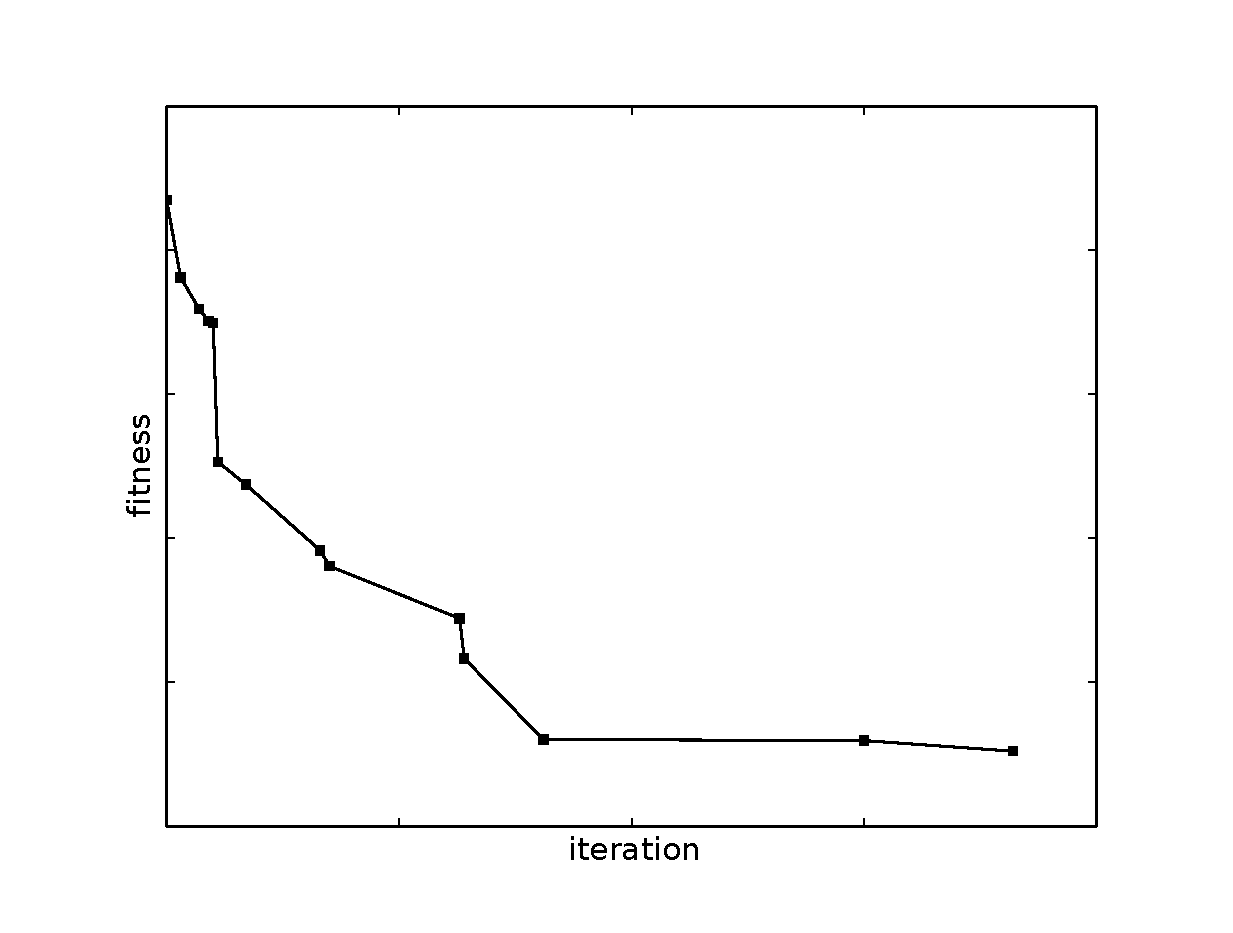
\includegraphics[width=5cm]{../paper/FIG/algo_hc}}
                    \caption*{Greedy approach to accept only fitter(low fitness) individuals}
                \end{figure}
            }
        \end{column}
    \end{columns}
\end{frame}

\begin{frame}{\null}
    \begin{tcolorbox}[colback=green!5]
        \centering\Huge
        Part 3: Evaluation of test cases
    \end{tcolorbox}
\end{frame}

\begin{frame}{Experimental Setup}
    \begin{enumerate}\itemsep1.2em
        \item All test cases describe platforms which are representative of real-world use cases like mobile devices, trucks, and cars. If one were to scale up we will expect same behaviour to hold
        \item We use a popular \textit{NEC2} simulator to get fitness parameters 
        \item Evaluated the entire search space using an exhaustive algorithm to find the optimal antenna locations which is not ordinarily possible
        \item Termination criteria was set to be at most $50\%$ evaluations of the search spcae
        \item $10$ independent runs of each test case against each algorithm with $\alpha = \beta = 1/2$
    \end{enumerate}
    \vspace{10mm}
\end{frame}


\begin{frame}{Experiments: Test Cases}
    \begin{columns}
        \begin{column}{.5\columnwidth}
            \begin{figure}
        \vspace*{-0.5cm}
                \centering
                \begin{subfigure}{\columnwidth}
                    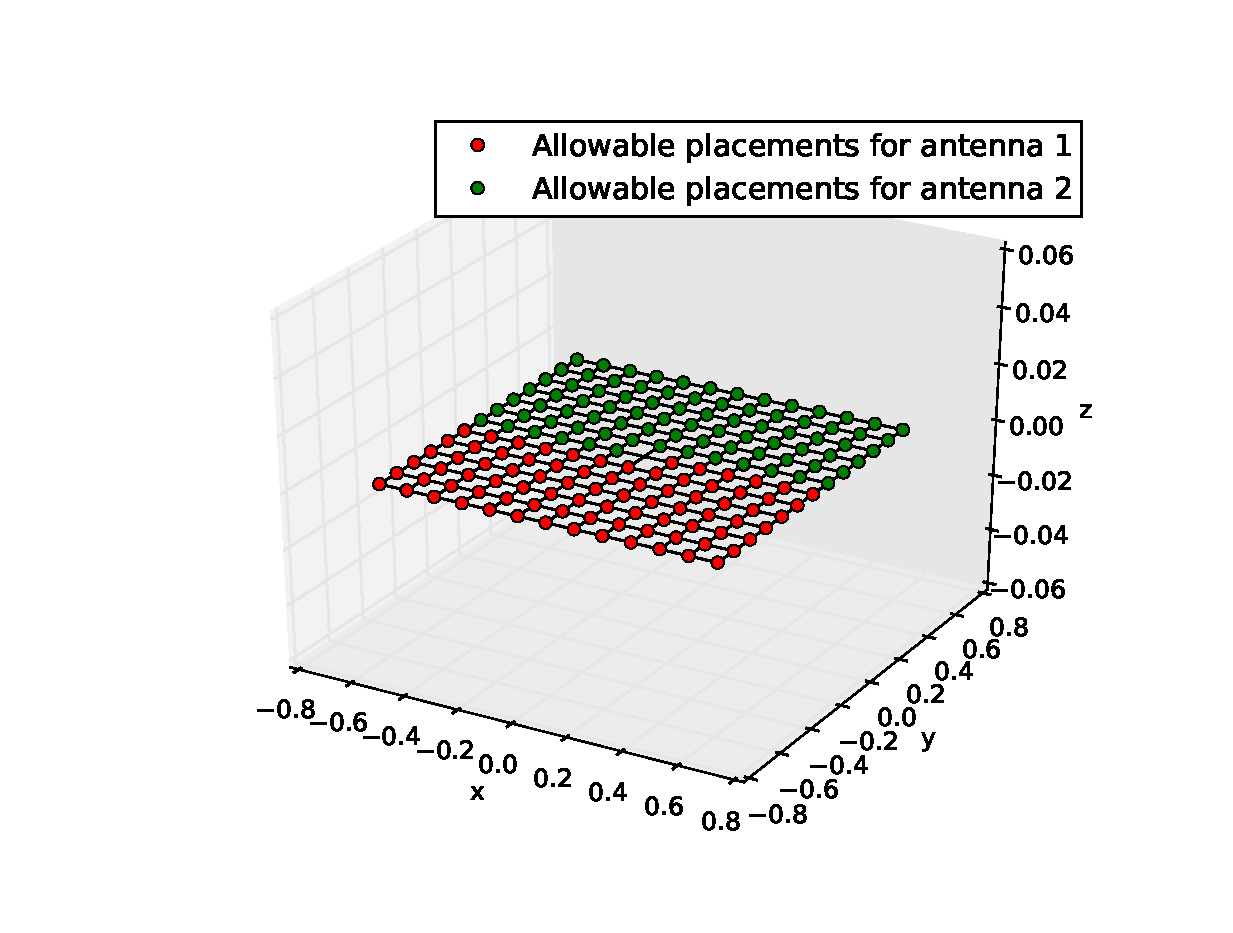
\includegraphics[trim=0 30 0 50, clip,scale=0.25]{../paper/FIG/tc1_figure}%
                    \caption*{\tiny Test Case \#1: search space size of $7056~(84x84)$ allowable placements}%
                \end{subfigure}\hfill\\
                \begin{subfigure}{\columnwidth}
                    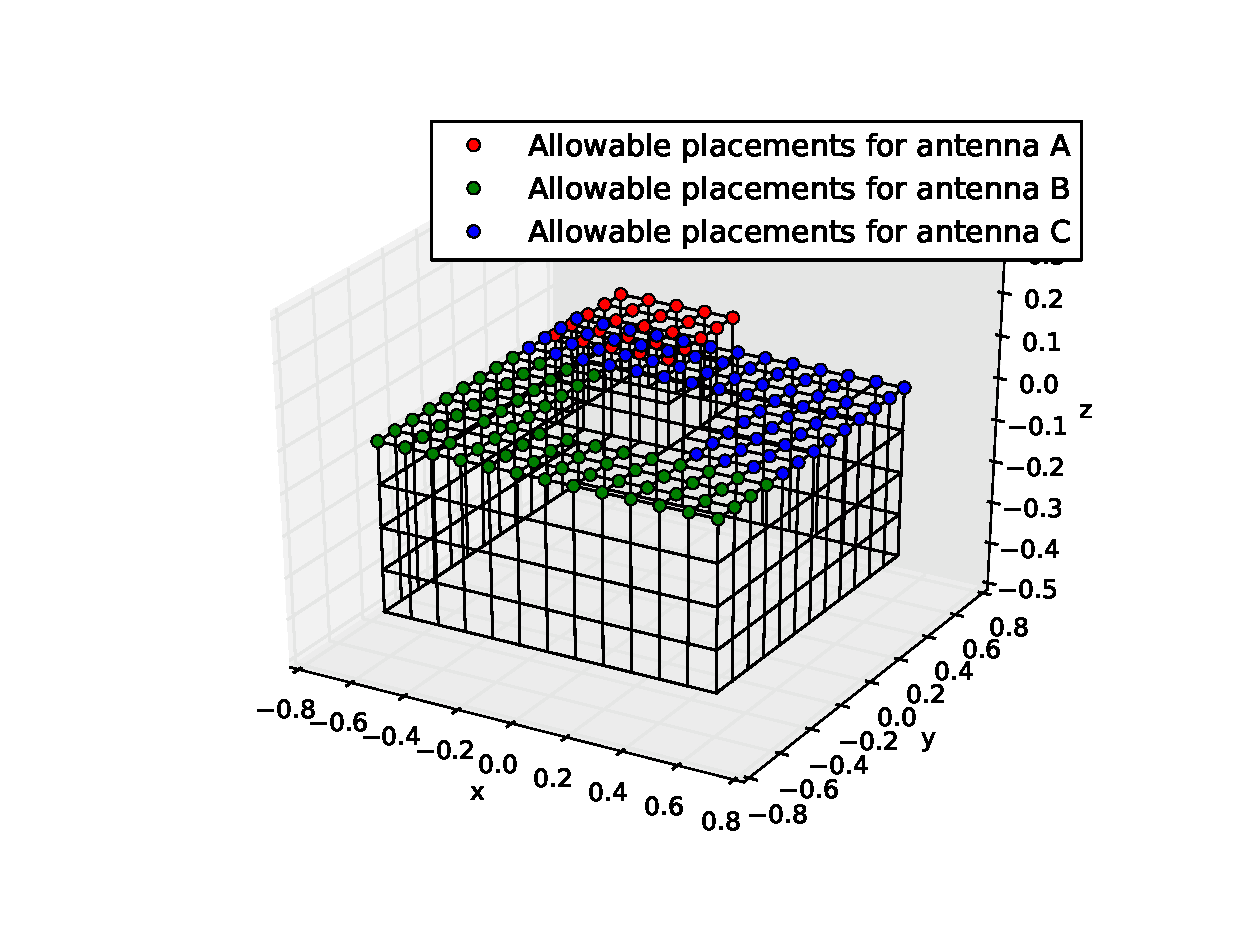
\includegraphics[trim=0 30 0 50, clip, scale=0.25]{../paper/FIG/tc3_figure}%
                    \caption*{\tiny Test Case \#3: search space size of $126025~(71x71x25)$ allowable placements}%
                \end{subfigure}\hfill%
            \end{figure}
        \end{column}
        \begin{column}{.5\columnwidth}
            \begin{figure}
                \vspace{-0.5cm}
                \begin{subfigure}{\columnwidth}
                    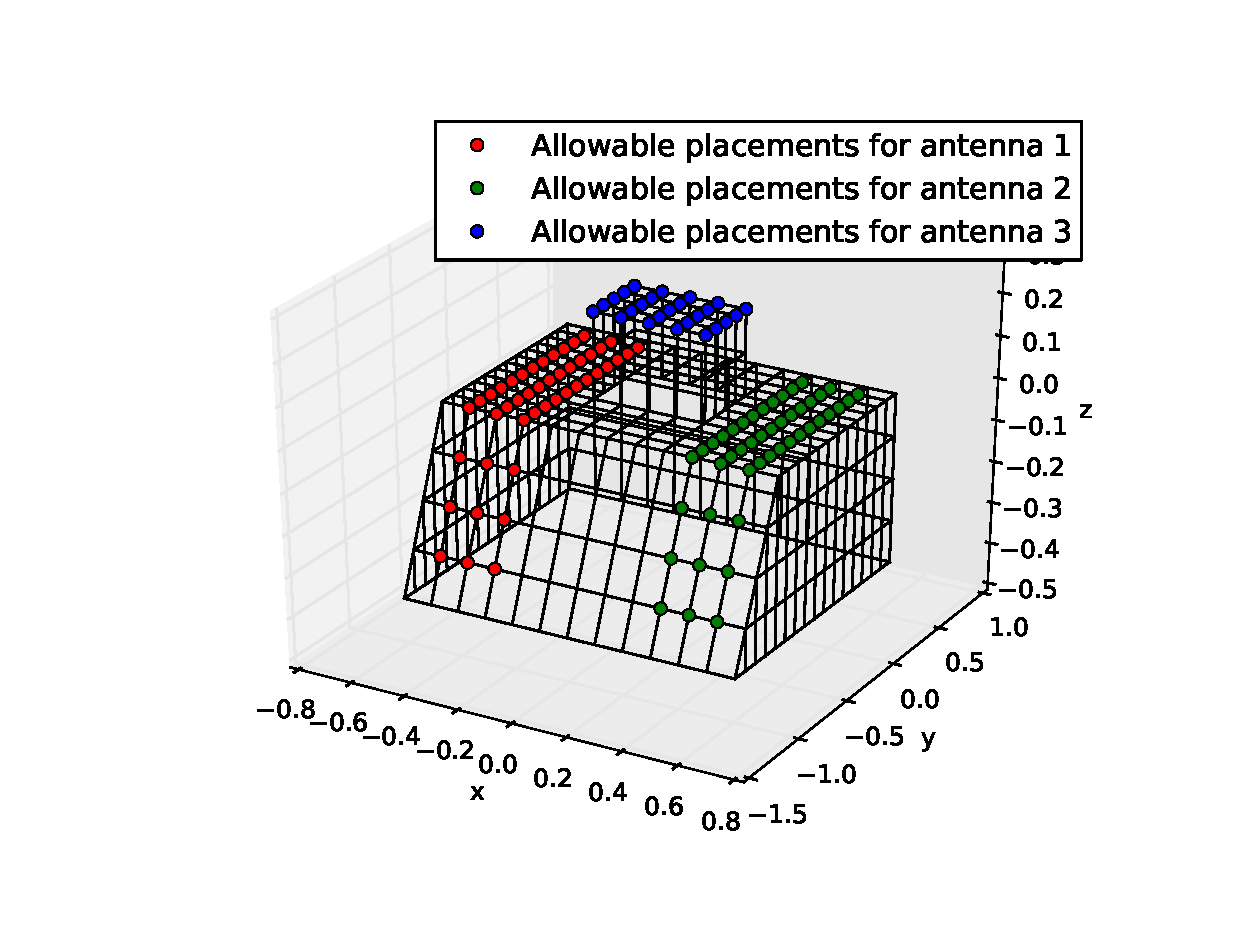
\includegraphics[trim=0 30 0 50, clip, scale=0.25]{../paper/FIG/tc2_figure}%
                    \caption*{\tiny Test Case \#2: search space size of $50625~(45x45x25)$ allowable placements}%
                \end{subfigure}\hfill\\%
                \begin{subfigure}{\columnwidth}
                    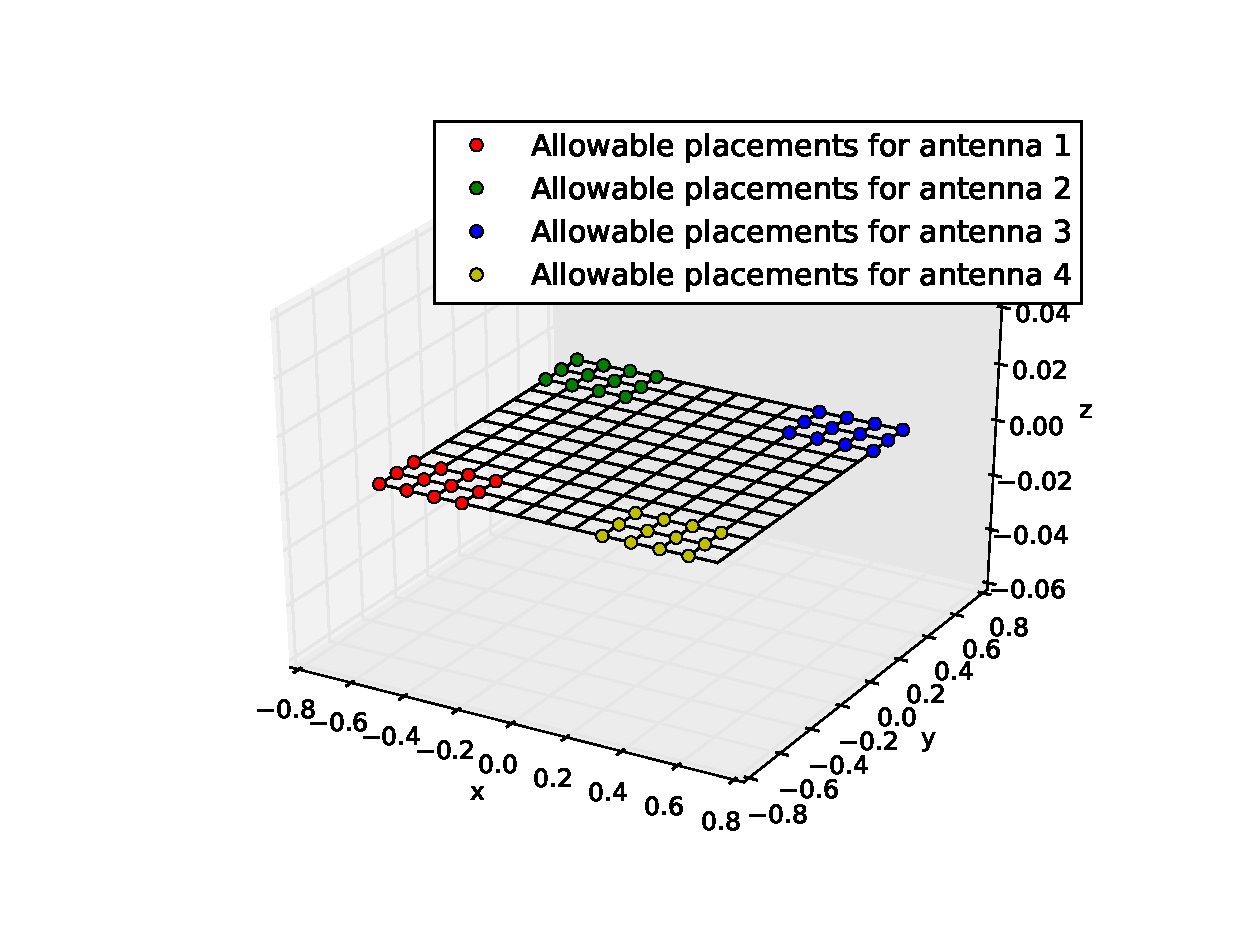
\includegraphics[trim=0 30 0 50, clip, scale=0.25]{../paper/FIG/tc4_figure}%
                    \caption*{\tiny Test Case \#4: search space size of $20736~(12x12x12x12)$ allowable placements}%
                \end{subfigure}\hfill%
            \end{figure}
        \end{column}
    \end{columns}
\end{frame}


\begin{frame}{Results - Test Case 1}
    \begin{figure}
        \centering
        \begin{subfigure}{.5\columnwidth}
            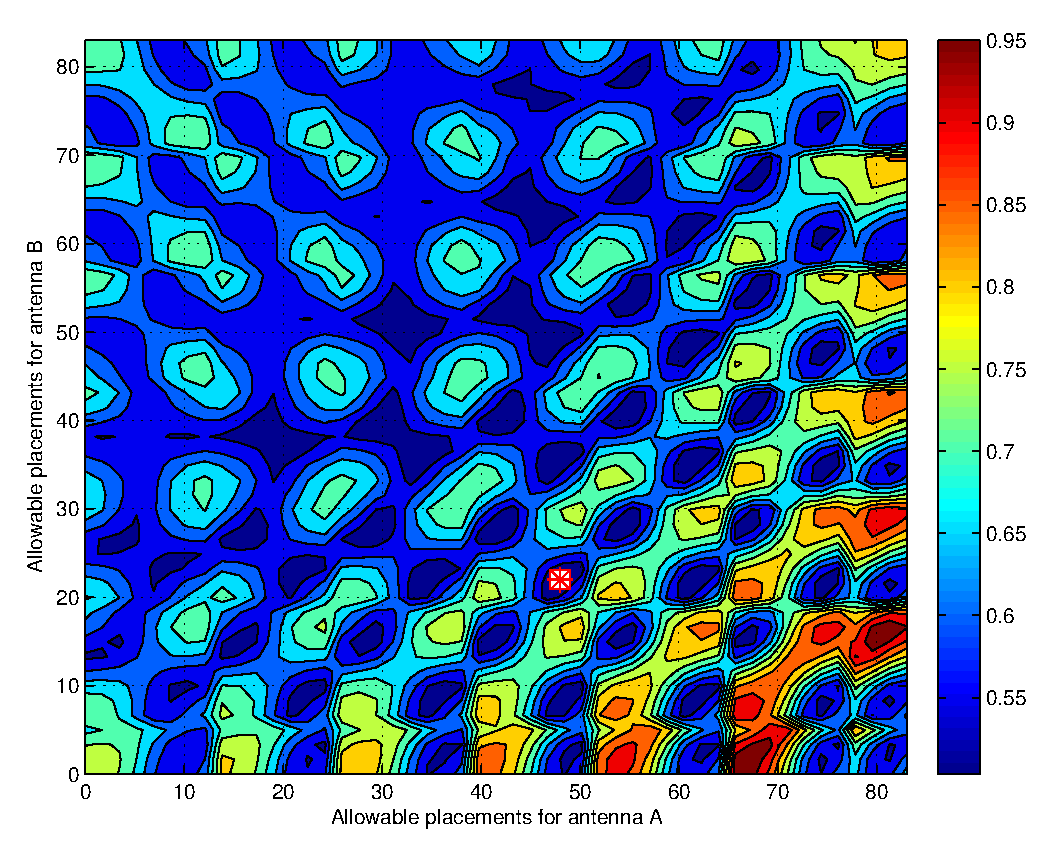
\includegraphics[width=\columnwidth,height=\columnwidth]{../paper/FIG/tc1_contour}%
        \end{subfigure}\hfill%
        \begin{subfigure}{.5\columnwidth}
            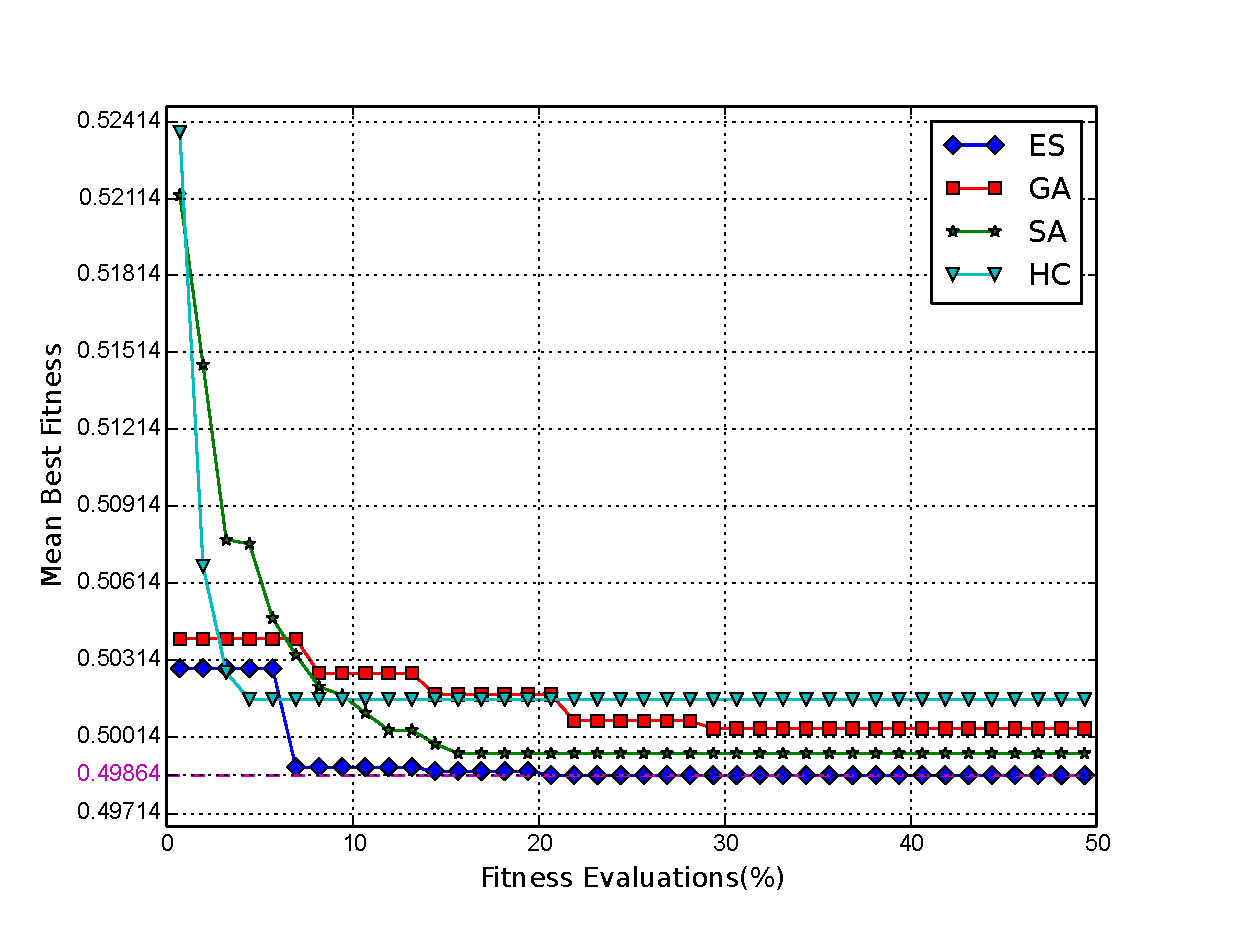
\includegraphics[width=\columnwidth, height=\columnwidth]{../paper/FIG/tc1_mf}%
        \end{subfigure}\hfill\\%
    \end{figure}
\end{frame}

\begin{frame}{Results - Test Case 2}
    \begin{figure}
        \centering
        \begin{subfigure}{.5\columnwidth}
            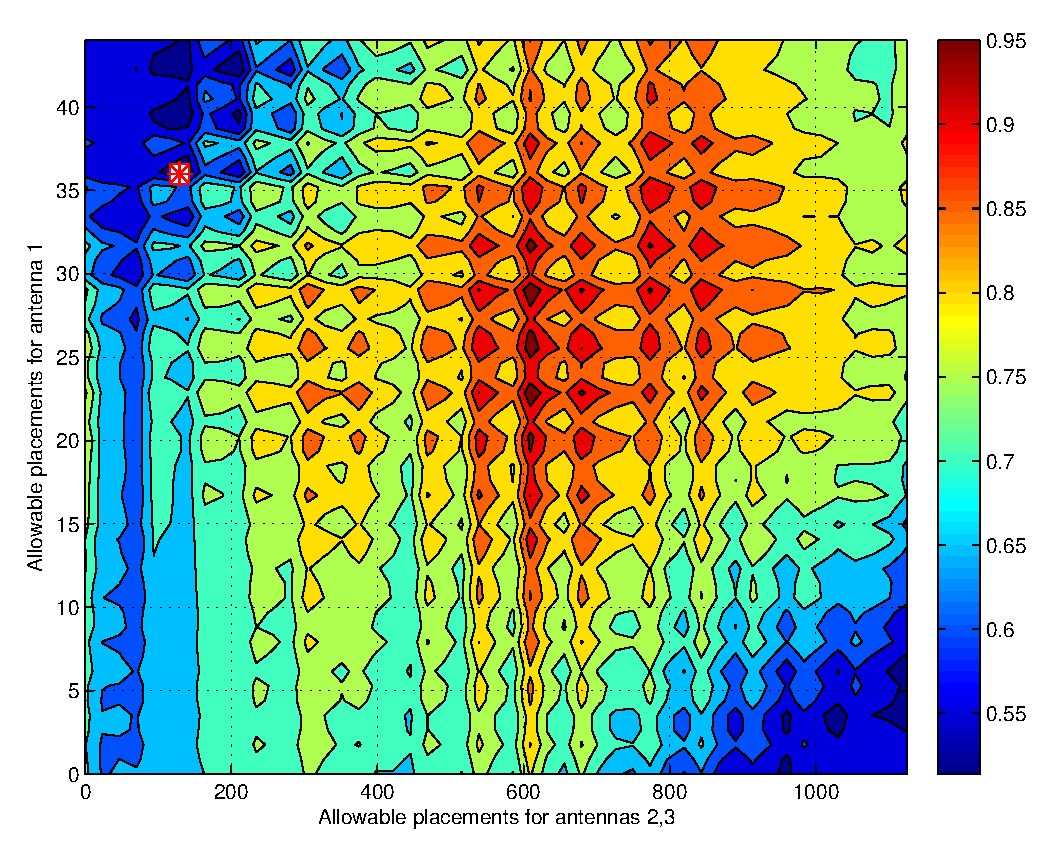
\includegraphics[width=\columnwidth,height=\columnwidth]{../paper/FIG/tc2_contour}%
        \end{subfigure}\hfill%
        \begin{subfigure}{.5\columnwidth}
            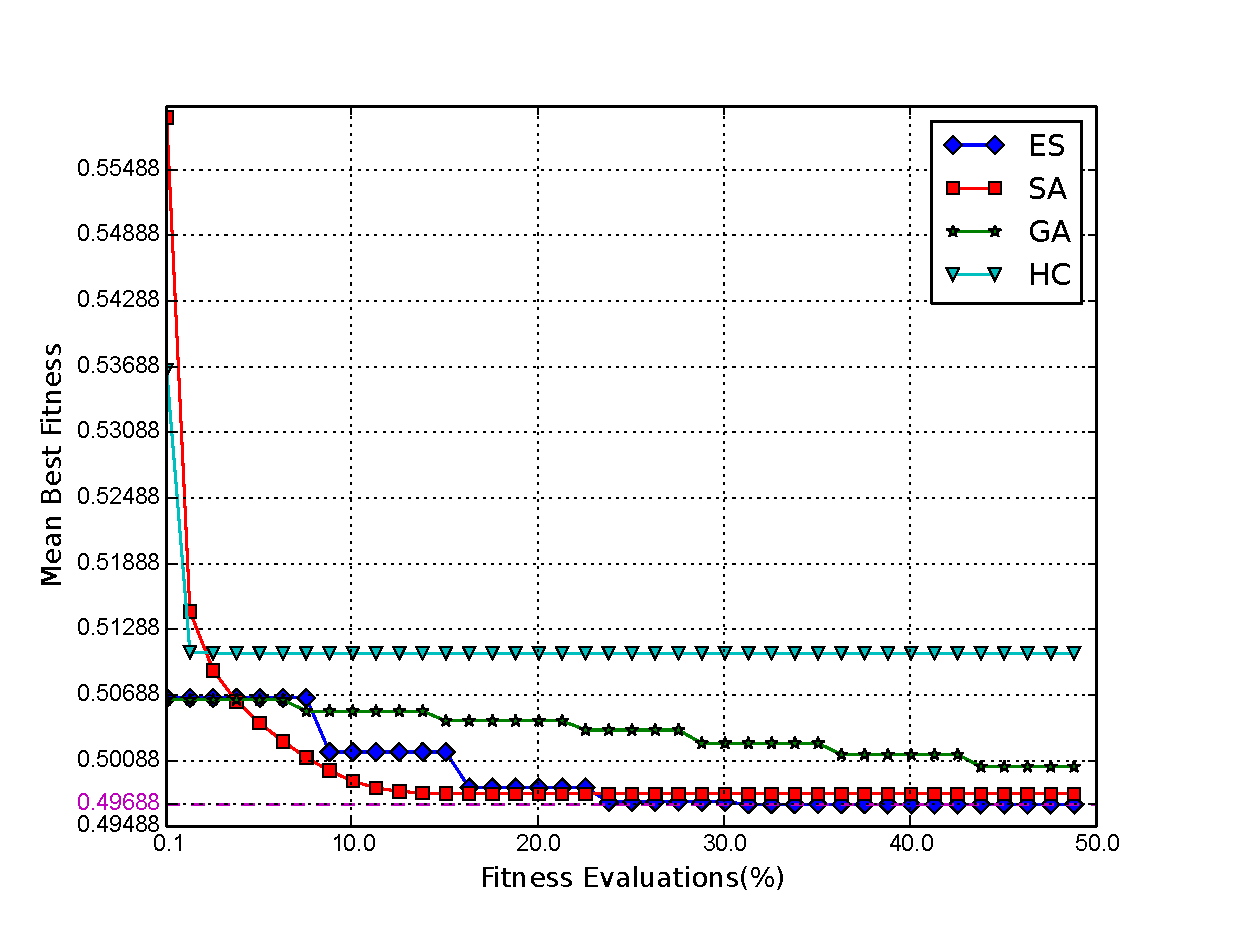
\includegraphics[width=\columnwidth, height=\columnwidth]{../paper/FIG/tc2_mf}%
        \end{subfigure}\hfill\\%
    \end{figure}
\end{frame}

\begin{frame}{Results - Test Case 3}
    \begin{figure}
        \centering
        \begin{subfigure}{.5\columnwidth}
            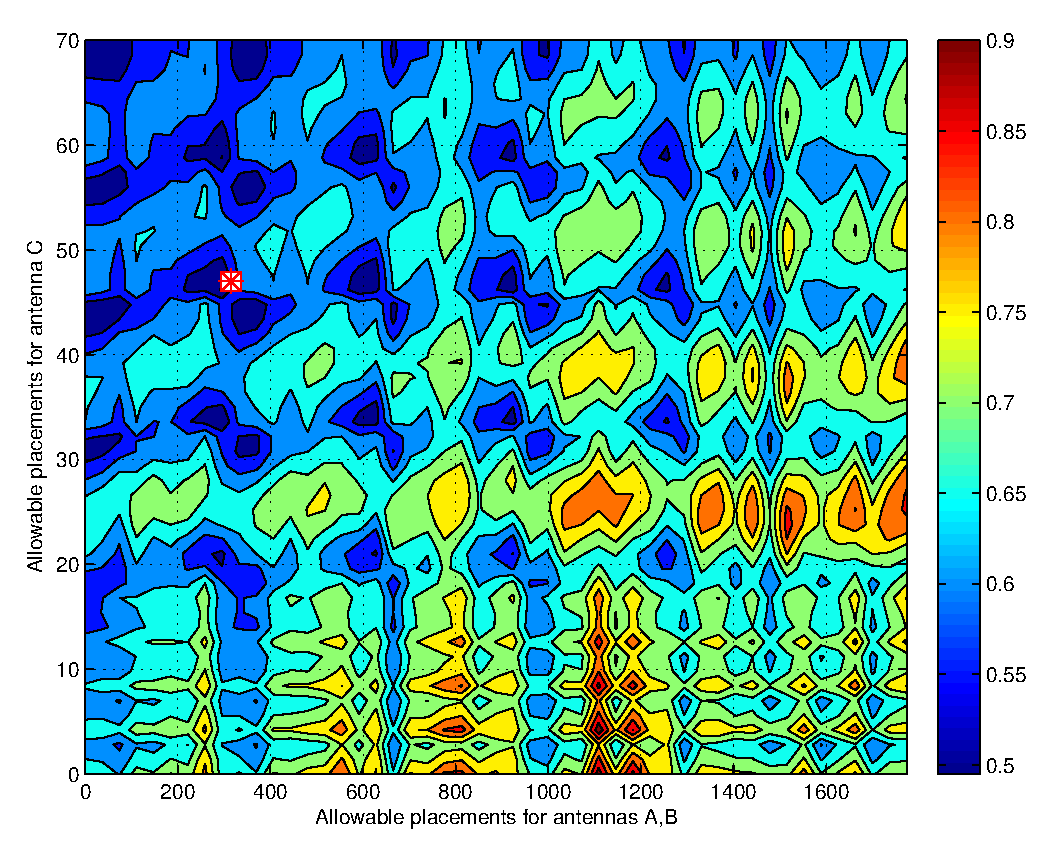
\includegraphics[width=\columnwidth,height=\columnwidth]{../paper/FIG/tc3_contour}%
        \end{subfigure}\hfill%
        \begin{subfigure}{.5\columnwidth}
            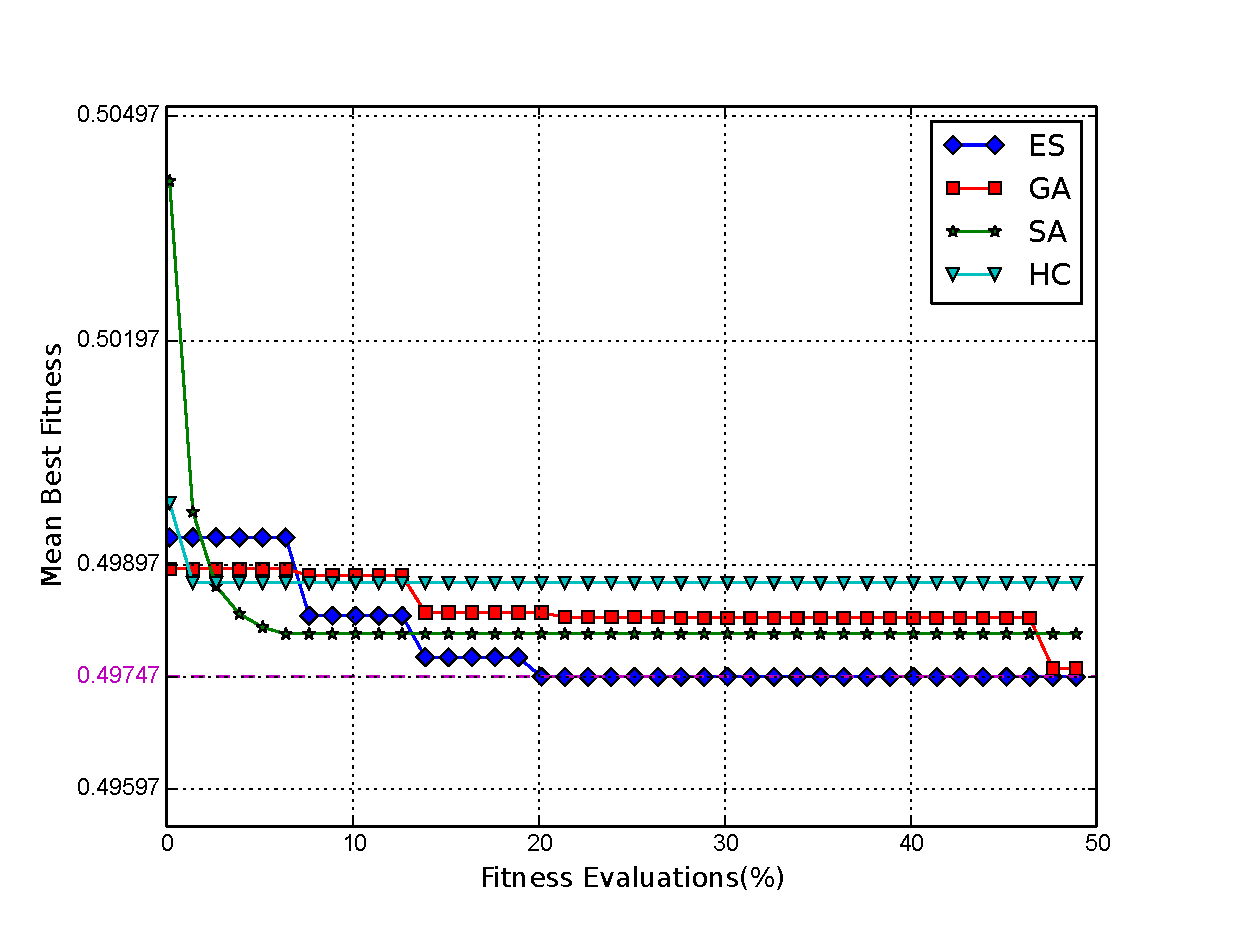
\includegraphics[width=\columnwidth, height=\columnwidth]{../paper/FIG/tc3_mf}%
        \end{subfigure}\hfill\\%
    \end{figure}
\end{frame}


\begin{frame}{Results - Test Case 4}
    \begin{figure}
        \centering
        \begin{subfigure}{.5\columnwidth}
            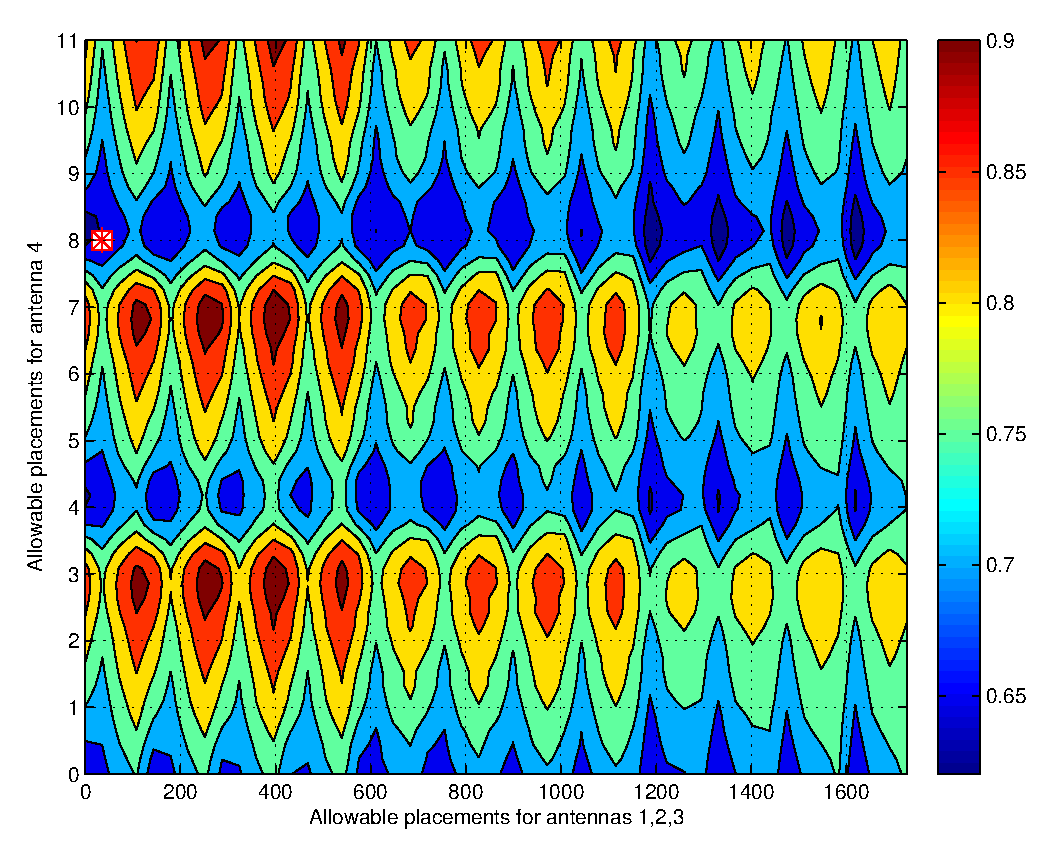
\includegraphics[width=\columnwidth,height=\columnwidth]{../paper/FIG/tc4_contour}%
        \end{subfigure}\hfill%
        \begin{subfigure}{.5\columnwidth}
            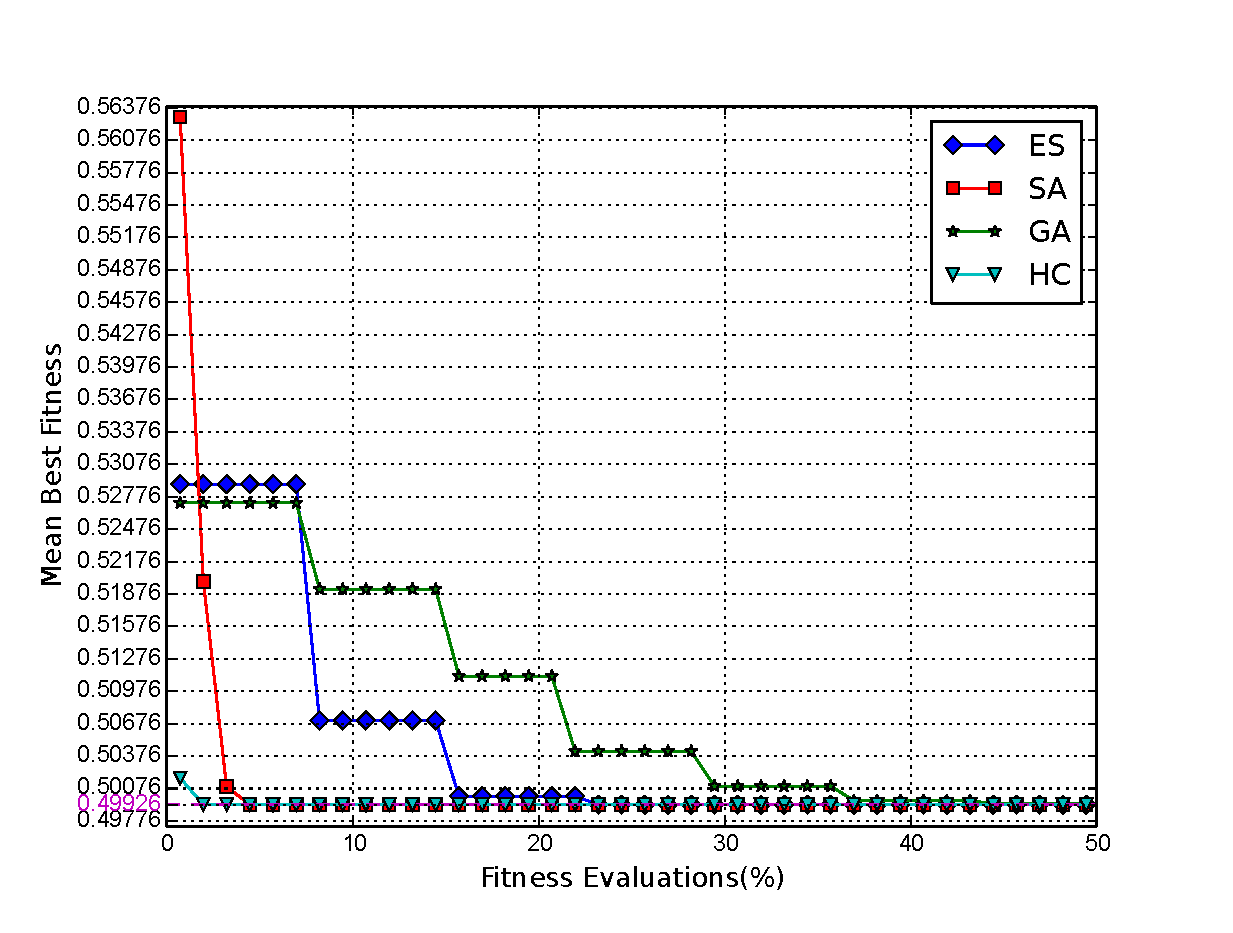
\includegraphics[width=\columnwidth, height=\columnwidth]{../paper/FIG/tc4_mf}%
        \end{subfigure}\hfill\\%
    \end{figure}
\end{frame}

\begin{frame}{Results - Success Rates}
    \textit{Success rate} report the percentage of runs in which the algorithm is able to find the optimum
    \begin{figure}
        \vspace*{-0.35cm}
        \centering
        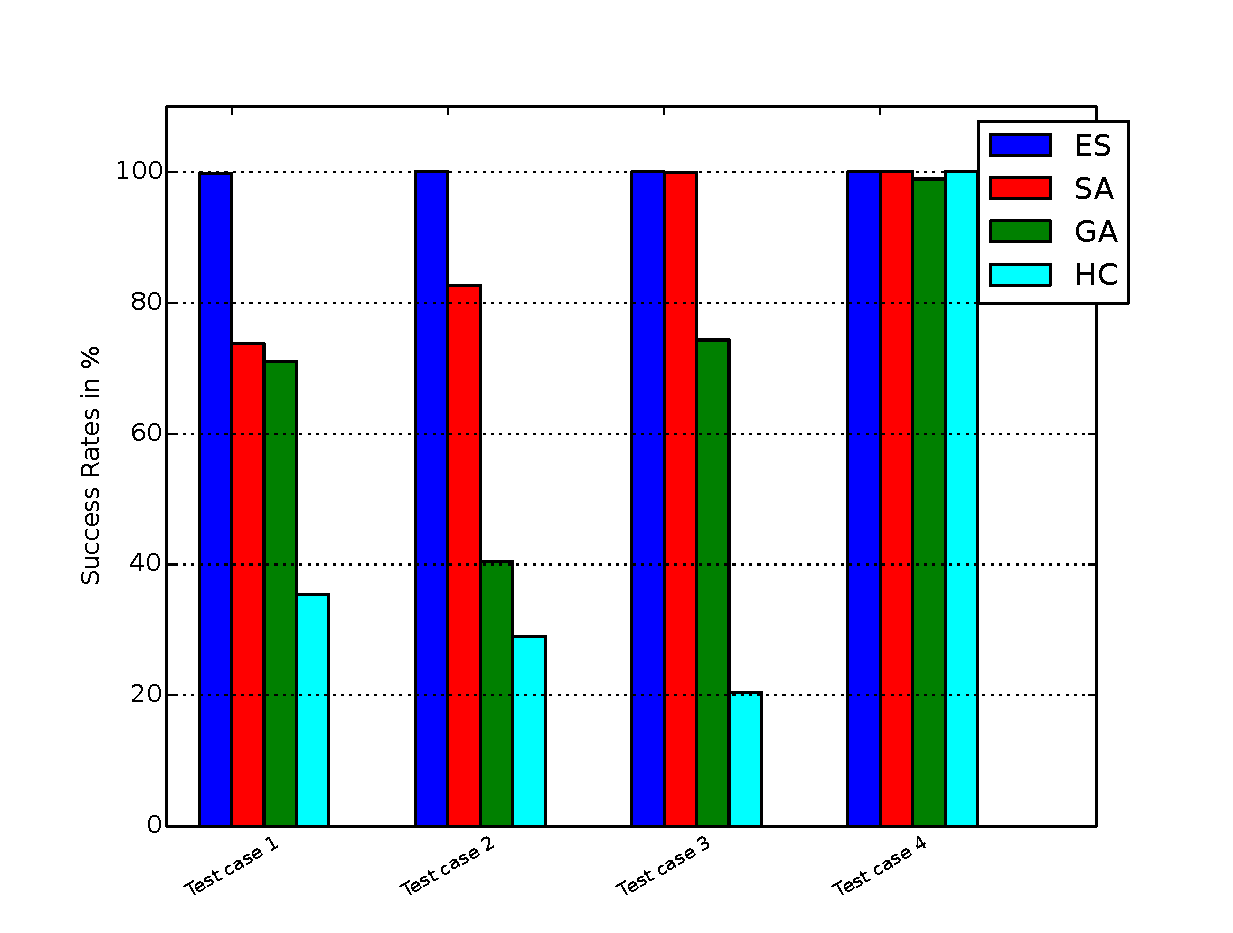
\includegraphics[scale=0.4]{../paper/FIG/tc_sp}
    \end{figure}
\end{frame}

\begin{frame}{Conclusion}
    \begin{itemize} \itemsep1.5em
        \item Formalized the antenna placement problem
        \item Generic problem formulation to accommodate multiple antennas and platforms
        \item Optimal placements found using Evolutionary Strategy with at most $25\%$ evaluations of search space
        % too weak, more numbers needed here
        \item Future work - Consider other techniques like \textit{Differential Evolution} and \textit{ALPS}
    \end{itemize}
\end{frame}

\end{document}
